\documentclass[11pt,letterpaper]{article}
\input{headings}
\usepackage{soul}
\newcommand \recipeName {Chocolate Passion}
\newcommand \fileName {ChocolatePassion}
\chead{\recipeName}

\begin{document}
\input{title}


This recipe was inspired on the individual small squares of cake covered with layers of mousses and a layer of jelly on top, called petit fours, that are typical in fancy French-style pastry shops. I prepared this for a dinner party and used old-style champagne stem glasses. The visual was very nice and several guests asked for seconds, and thirds.
	
\begin{description}
\item[Ingredients:]\ \\
	\begin{itemize}
	\item 1 recipe of \href{ChocolateMousse.html}{Chocolate Mousse}
	\item  1 recipe of \href{PassionFruitMousse.html}{Passion Fruit Mousse}
	\item 225 ml of apricot jelly (French style)
	\item 3/4 cup of passion fruit mousse
	\end{itemize}

	\begin{enumerate}
	\item {\bf Prepare the chocolate base}
		\begin{itemize}
		\item Prepare the chocolate mousse according to master recipe and fill the containers up to a little below half.
		\item Put in the refrigerator to cool off for about 1/2 hour --- this prevents condensation from forming.
		\item Cover the containers with plastic wrap to prevent drying too much in the refrigerator and put back into the refrigerator for the chocolate mousse to set completely.
		\end{itemize}

	\item {\bf Prepare the passion-fruit layer}
		\begin{itemize}
		\item Prepare the passion-fruit mousse according to master recipe.
                \item Remove the containers from the refrigerator, carefully remove the plastic covers.
                \item Pour on top of the chocolate mousse leaving a small space on the top for the jelly layer.
		\item Put, uncovered, in the refrigerator to cool off for about 1/2 hour --- this prevents condensation from forming.
		\item Cover the containers with plastic wrap to prevent drying too much in the refrigerator and put back into the refrigerator for the passion-fruit mousse to set completely.
		\end{itemize}
	\item {\bf Prepare the jelly top layer}
		\begin{itemize}
		\item Pour the apricot jelly into a small sauce pan and warm up over moderate heat until it is warmed through.
		\item Remove from the stove and add 1/2 cup of the passion-fruite juice (reserve the remaining 1/4 cup).
                \item Put a sieve on top of a bowl and pass the jelly and juice combination through the sieve to strain any solids.
		\item Let it cool off to room temperature on top of the counter.
                \item Stir the 1/4 cup of passion-fruit juice.
                \item At serving time, remove the containers from the refrigerator, put one tablespoon of the jelly-juice combination on top of each container and rotate the container around in your hand to distribute the jelly layer on top. 
		\end{itemize}	
		\end{enumerate}
\end{description}
\begin{table}
\begin{tabular}{cccc}
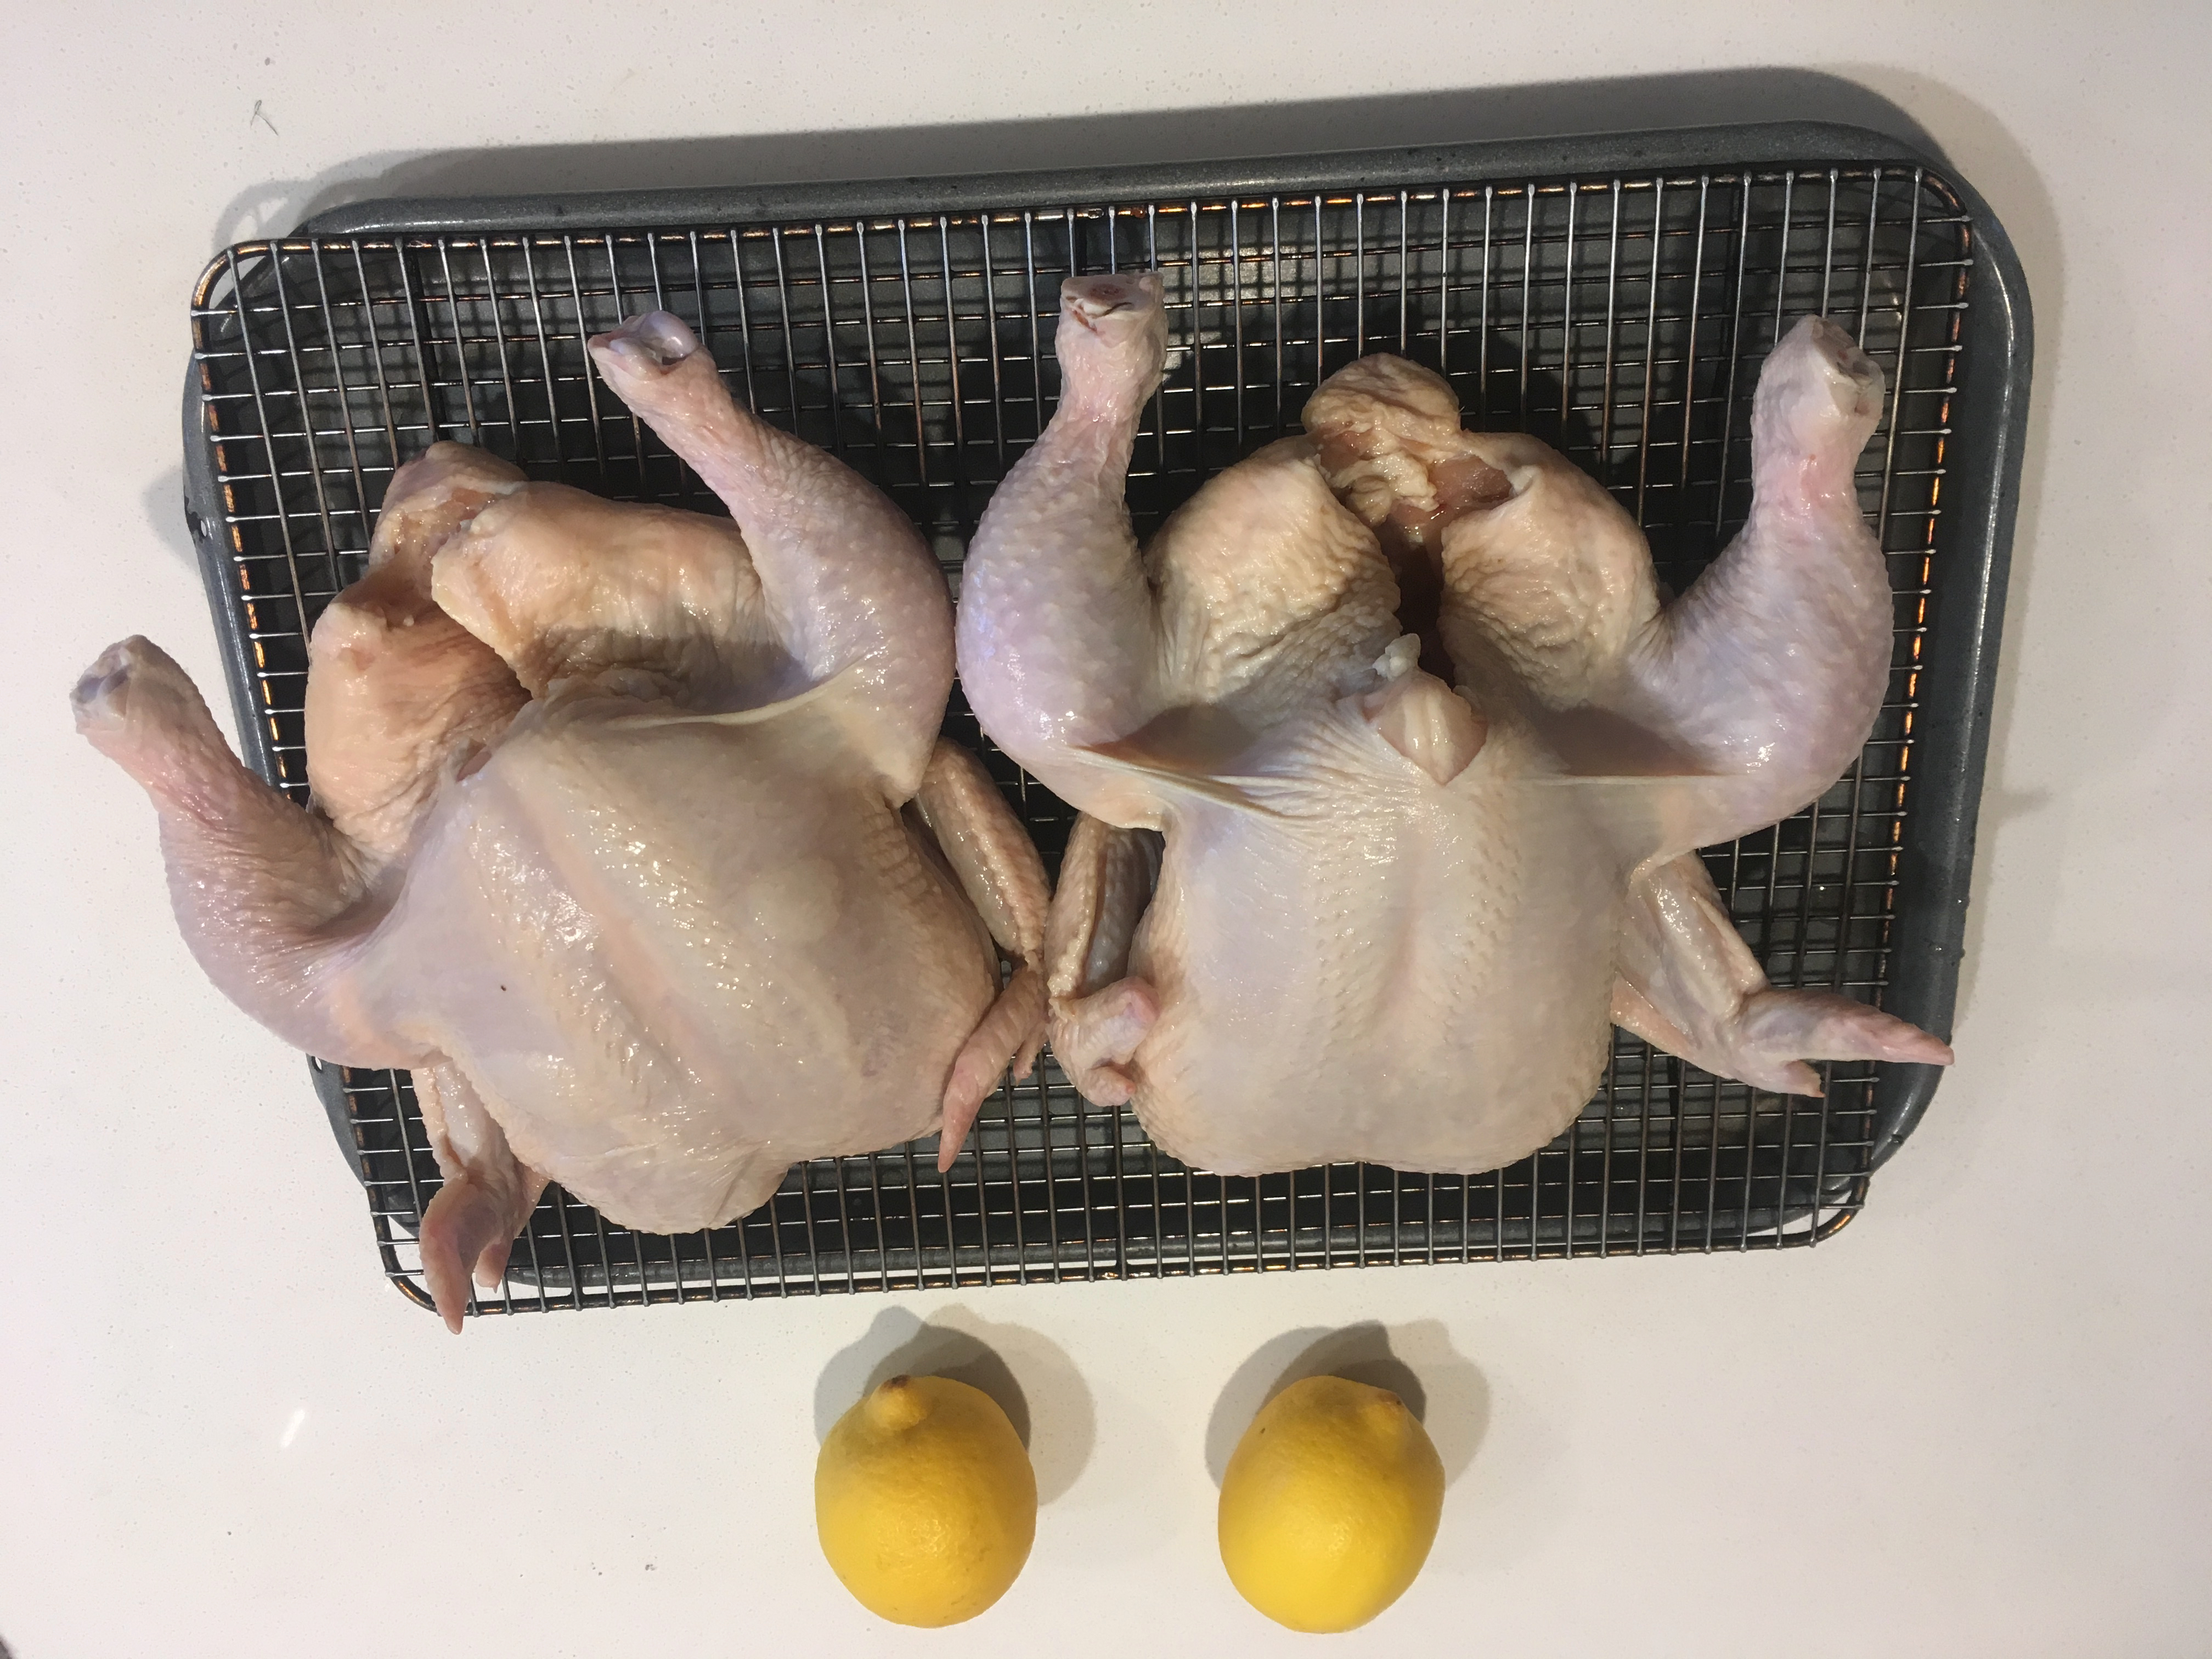
\includegraphics[width=0.25\textwidth]{\imageDir/\fileName/IMG_3197.jpg} &
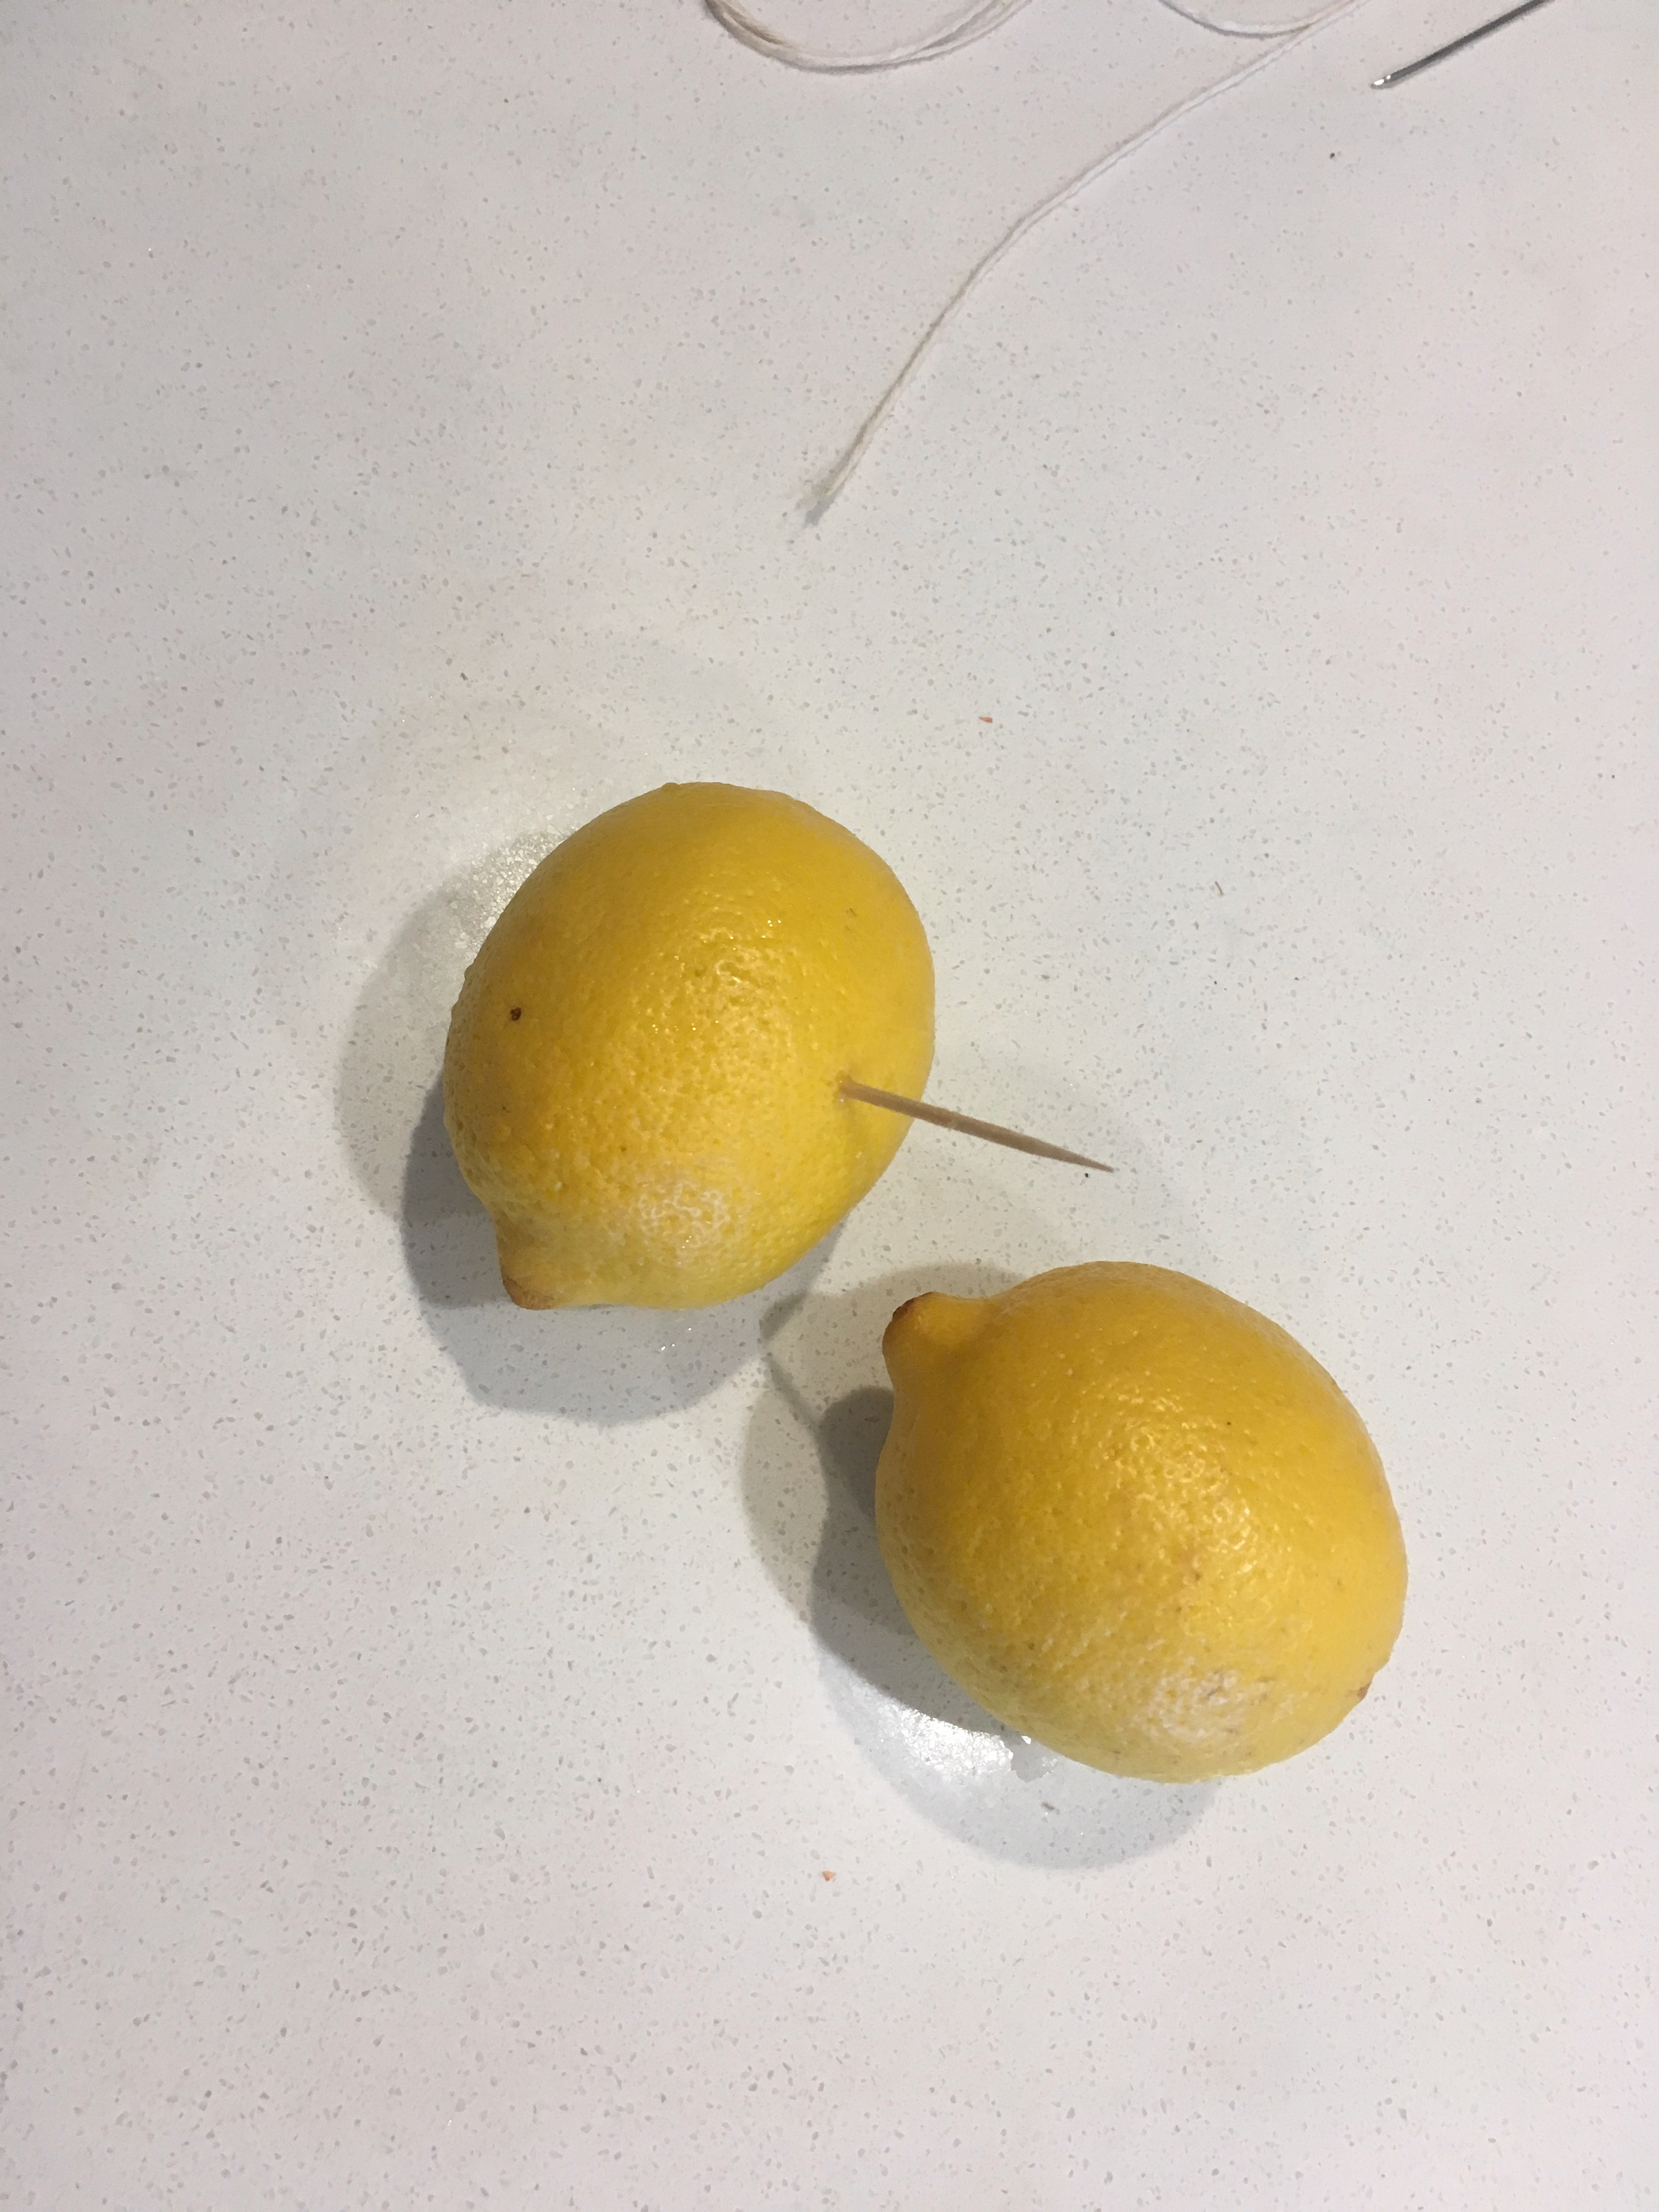
\includegraphics[width=0.25\textwidth]{\imageDir/\fileName/IMG_3212.jpg} &
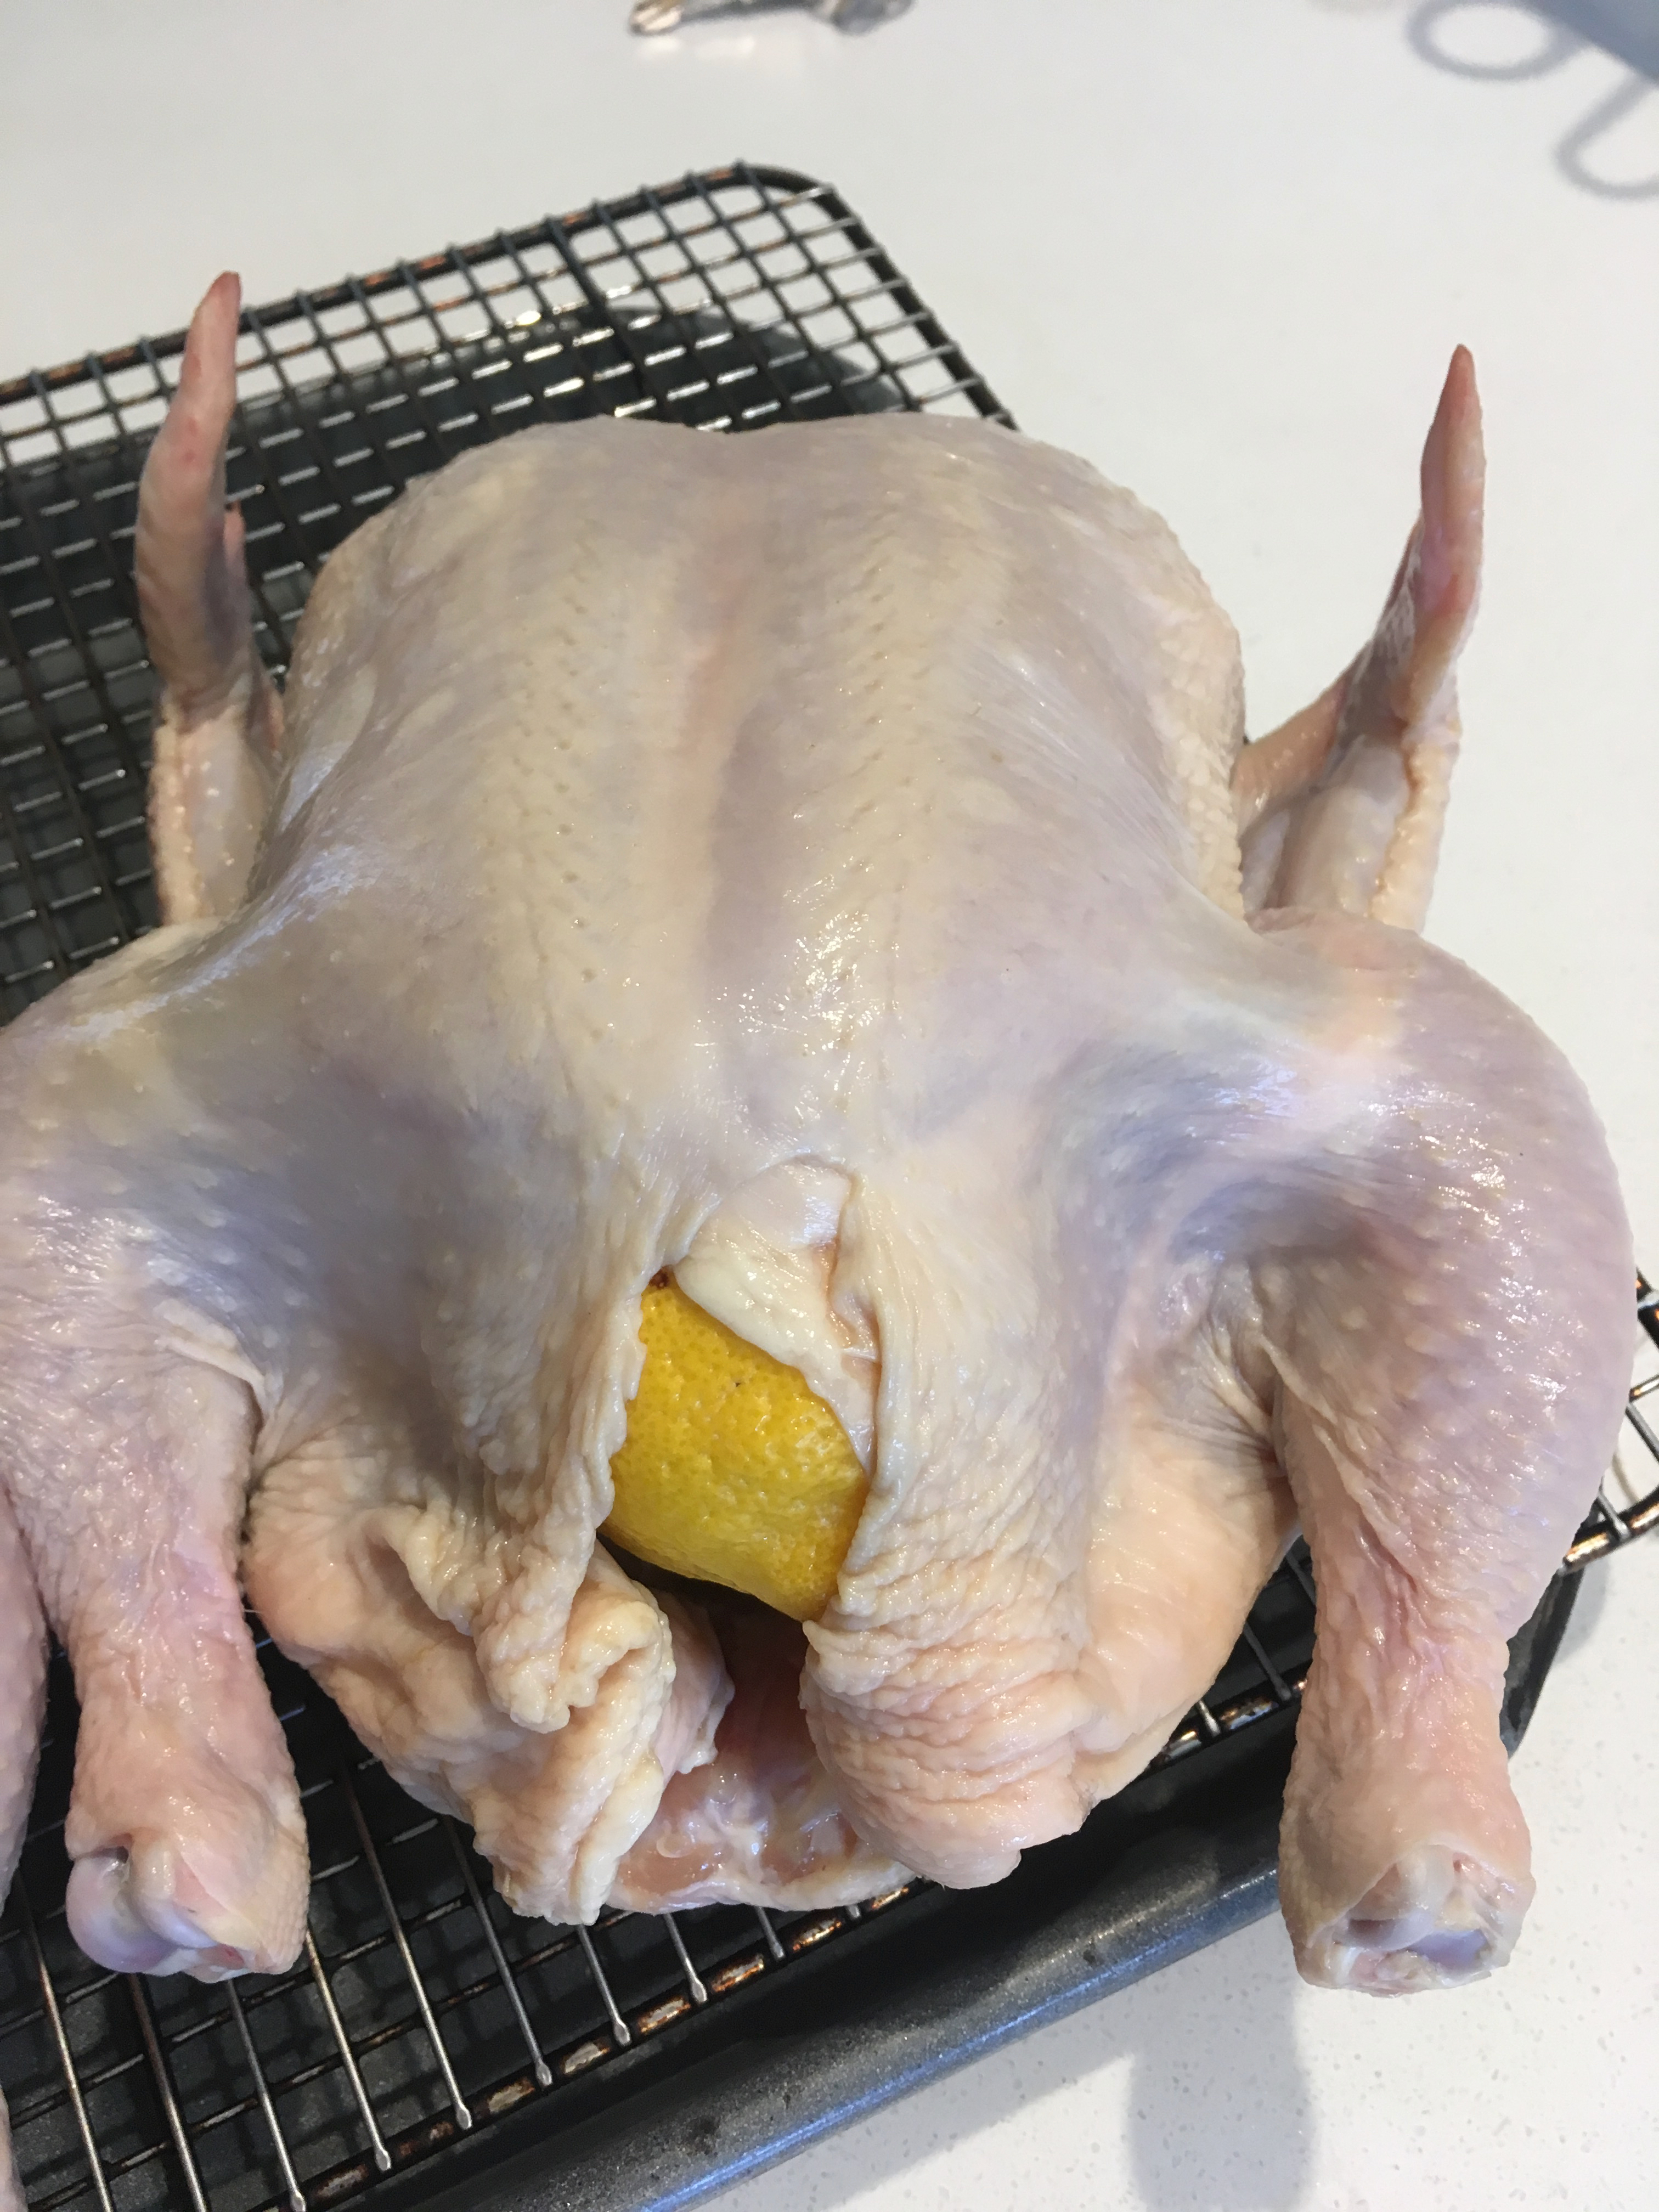
\includegraphics[width=0.25\textwidth]{\imageDir/\fileName/IMG_3213.jpg} \\
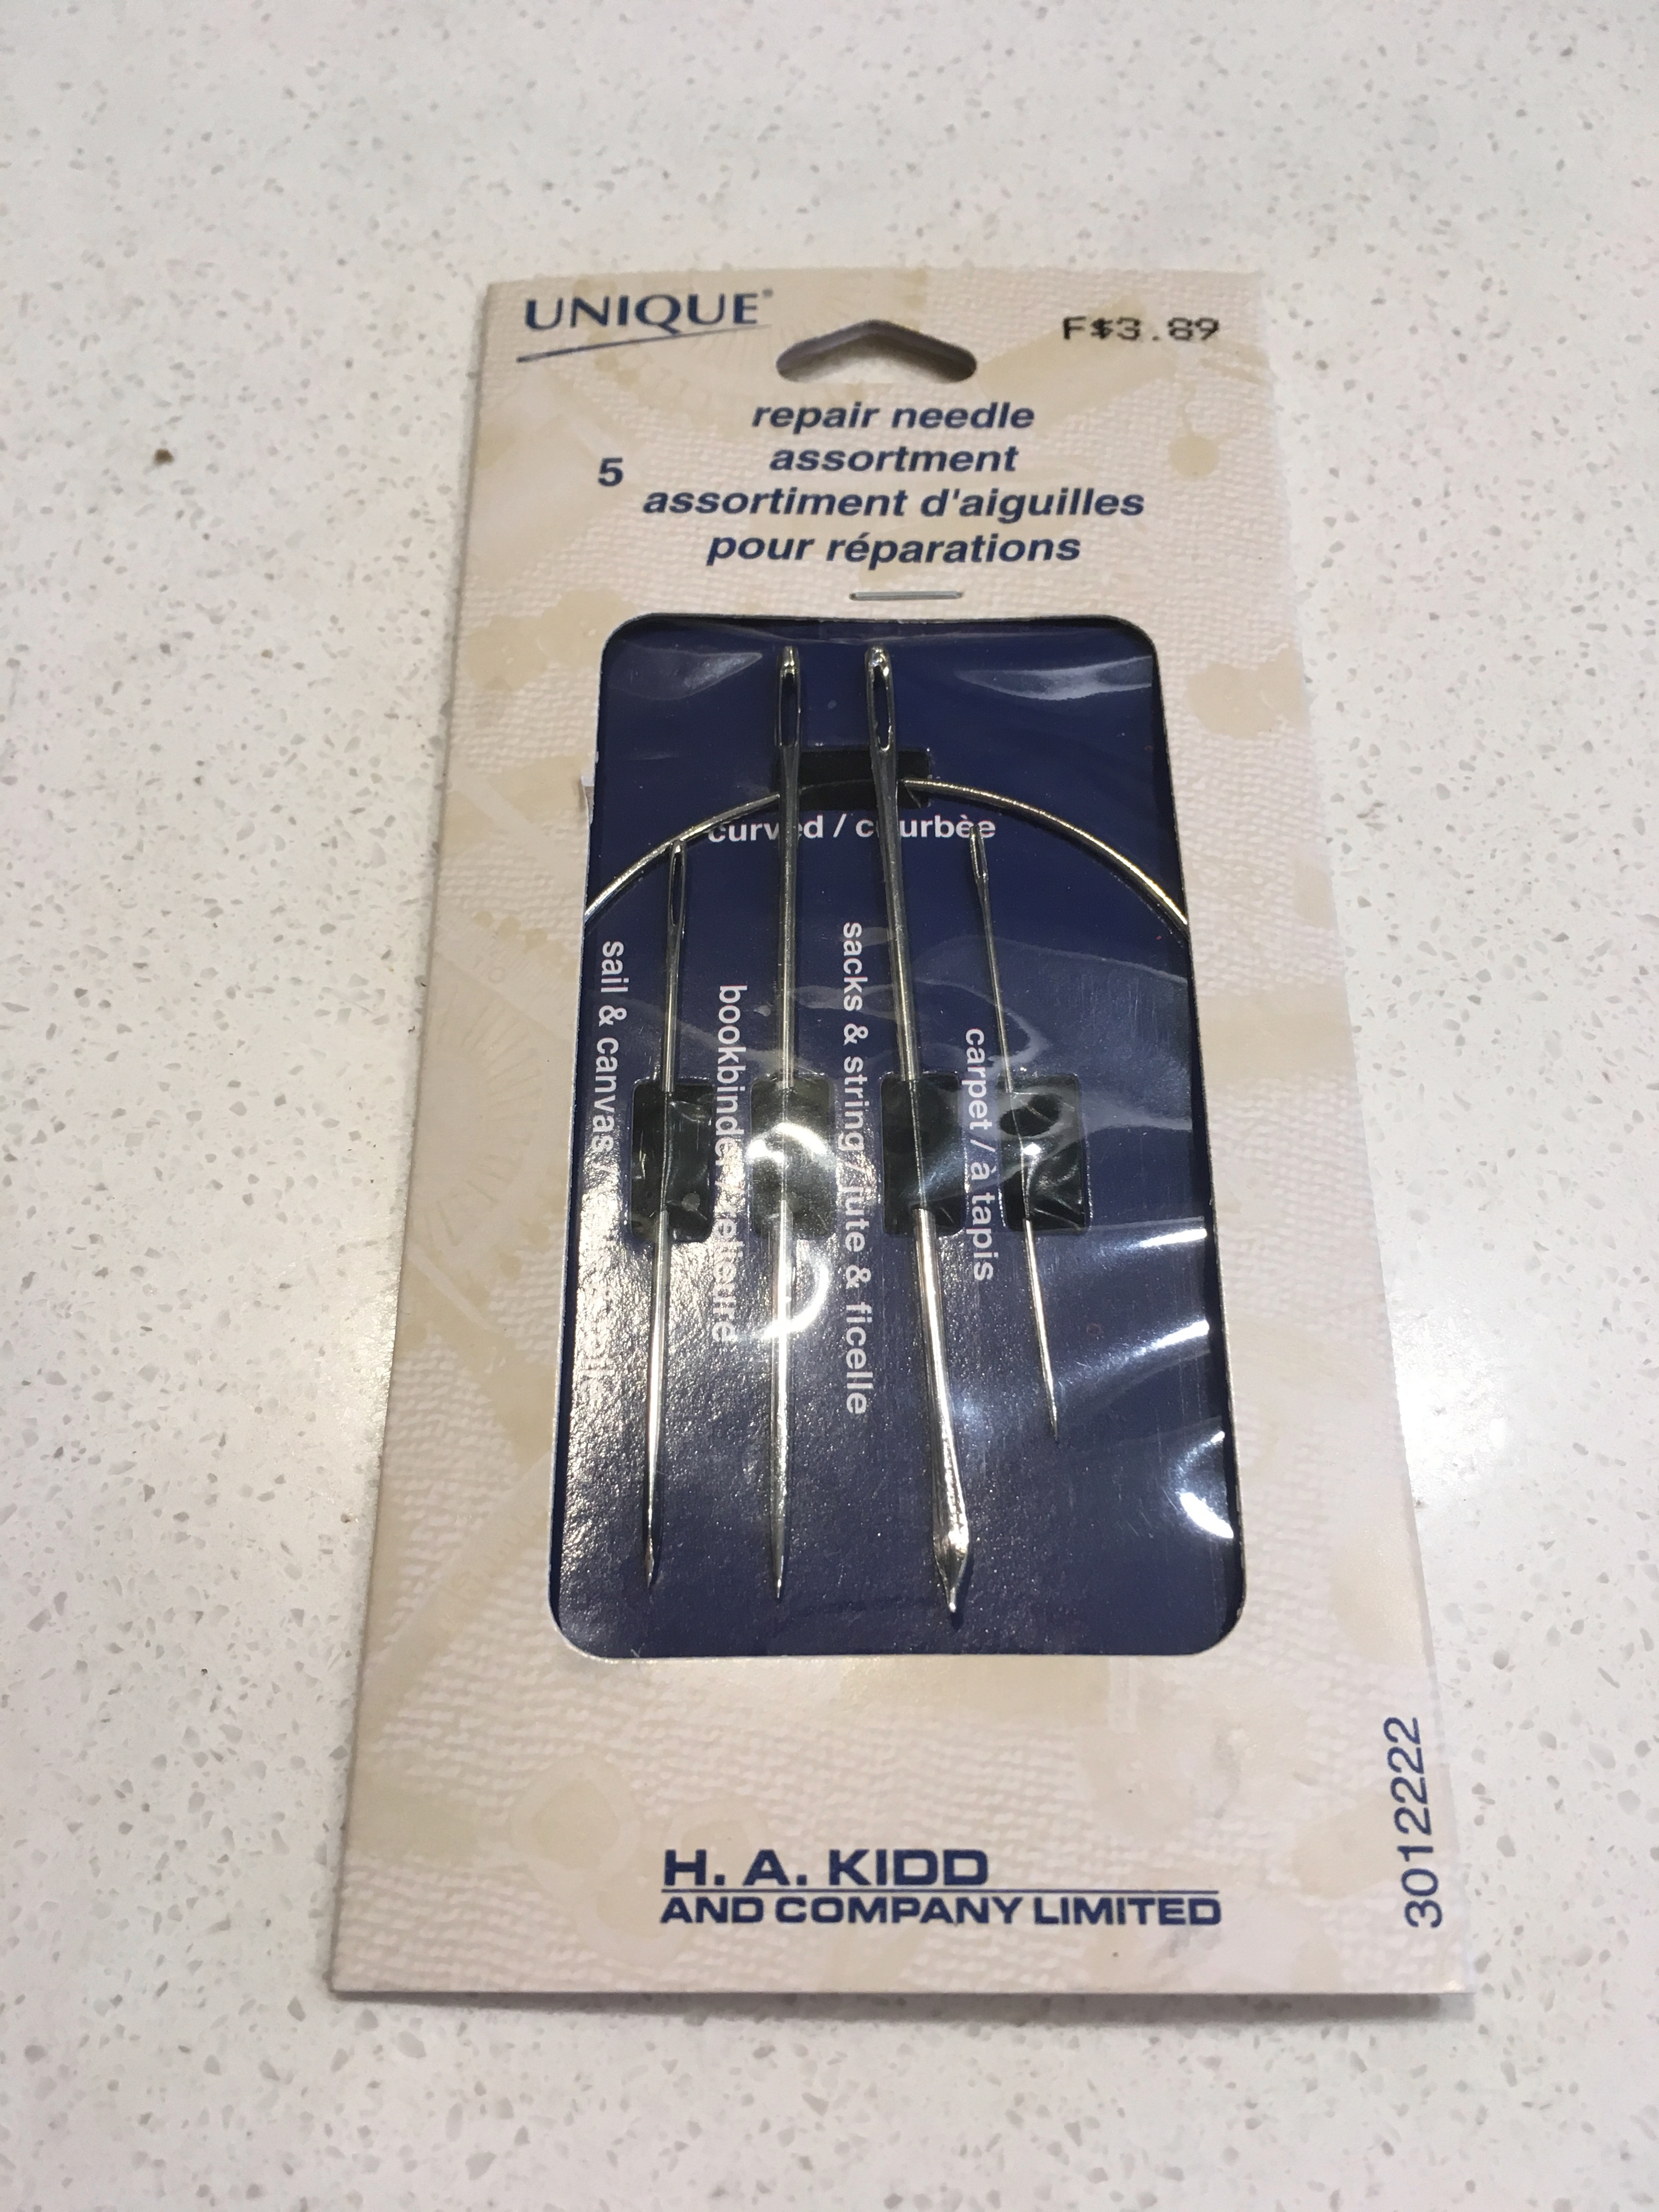
\includegraphics[width=0.25\textwidth]{\imageDir/\fileName/IMG_3206.jpg} &
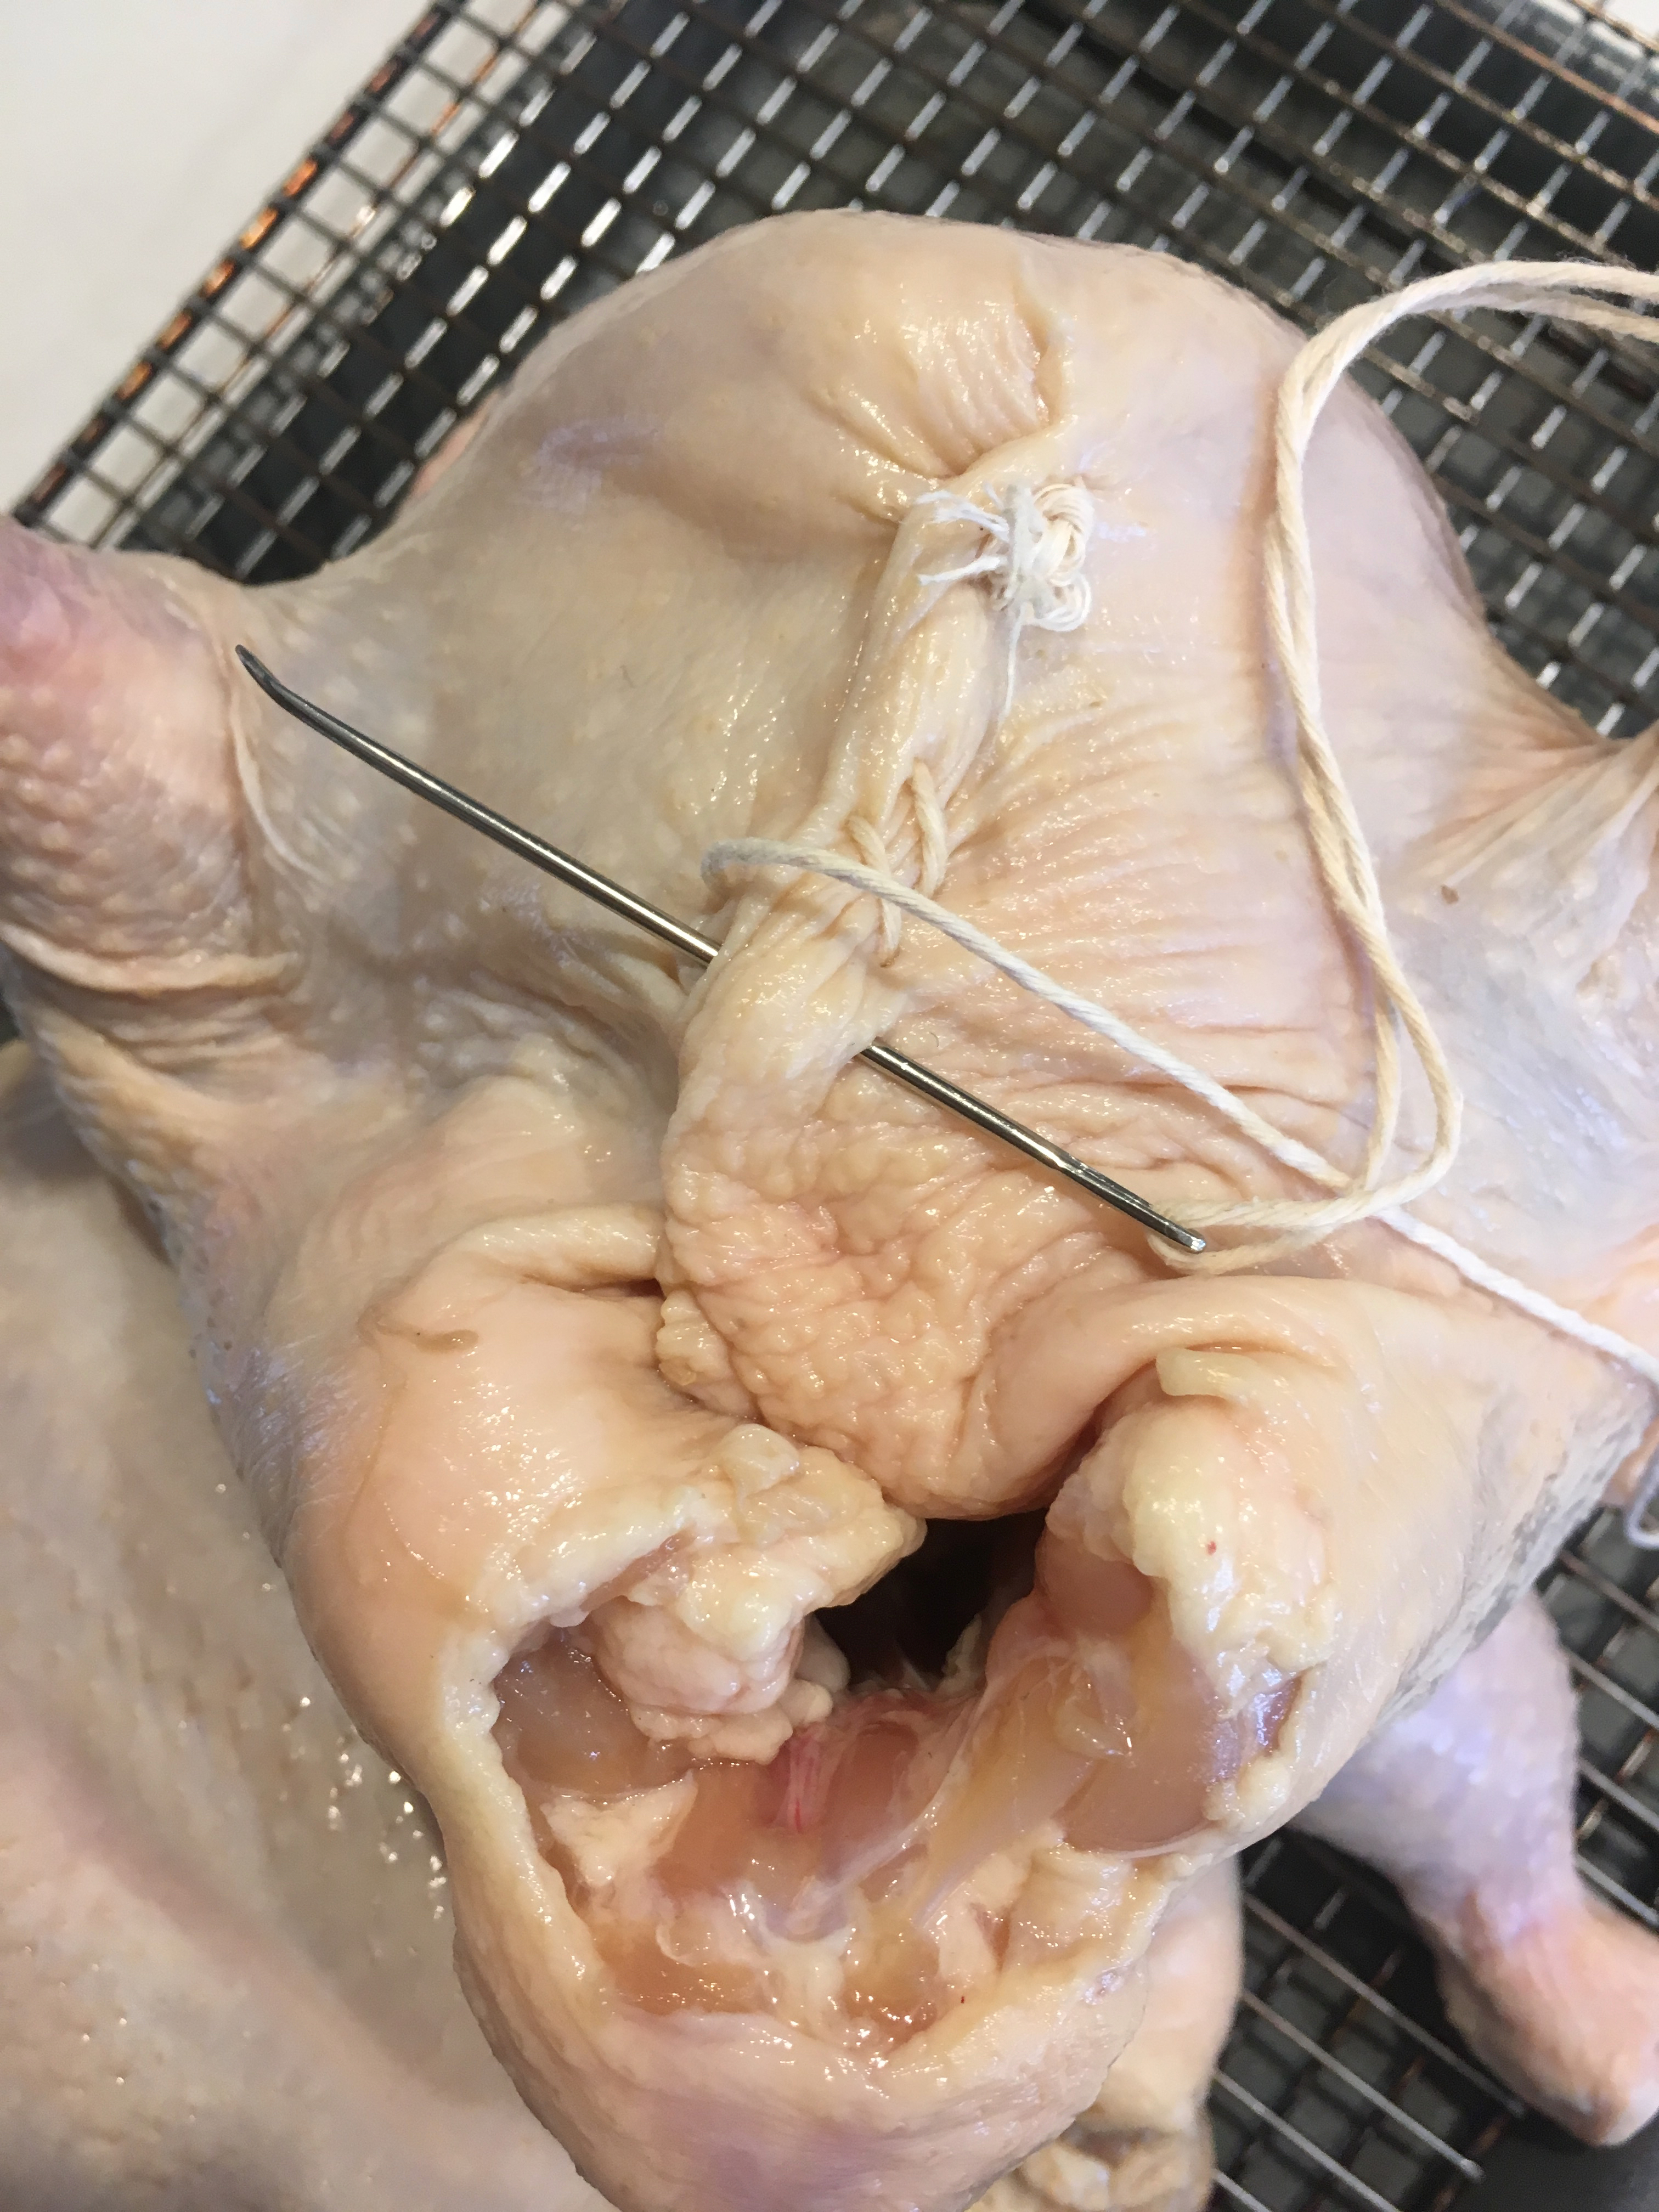
\includegraphics[width=0.25\textwidth]{\imageDir/\fileName/IMG_3214.jpg} &
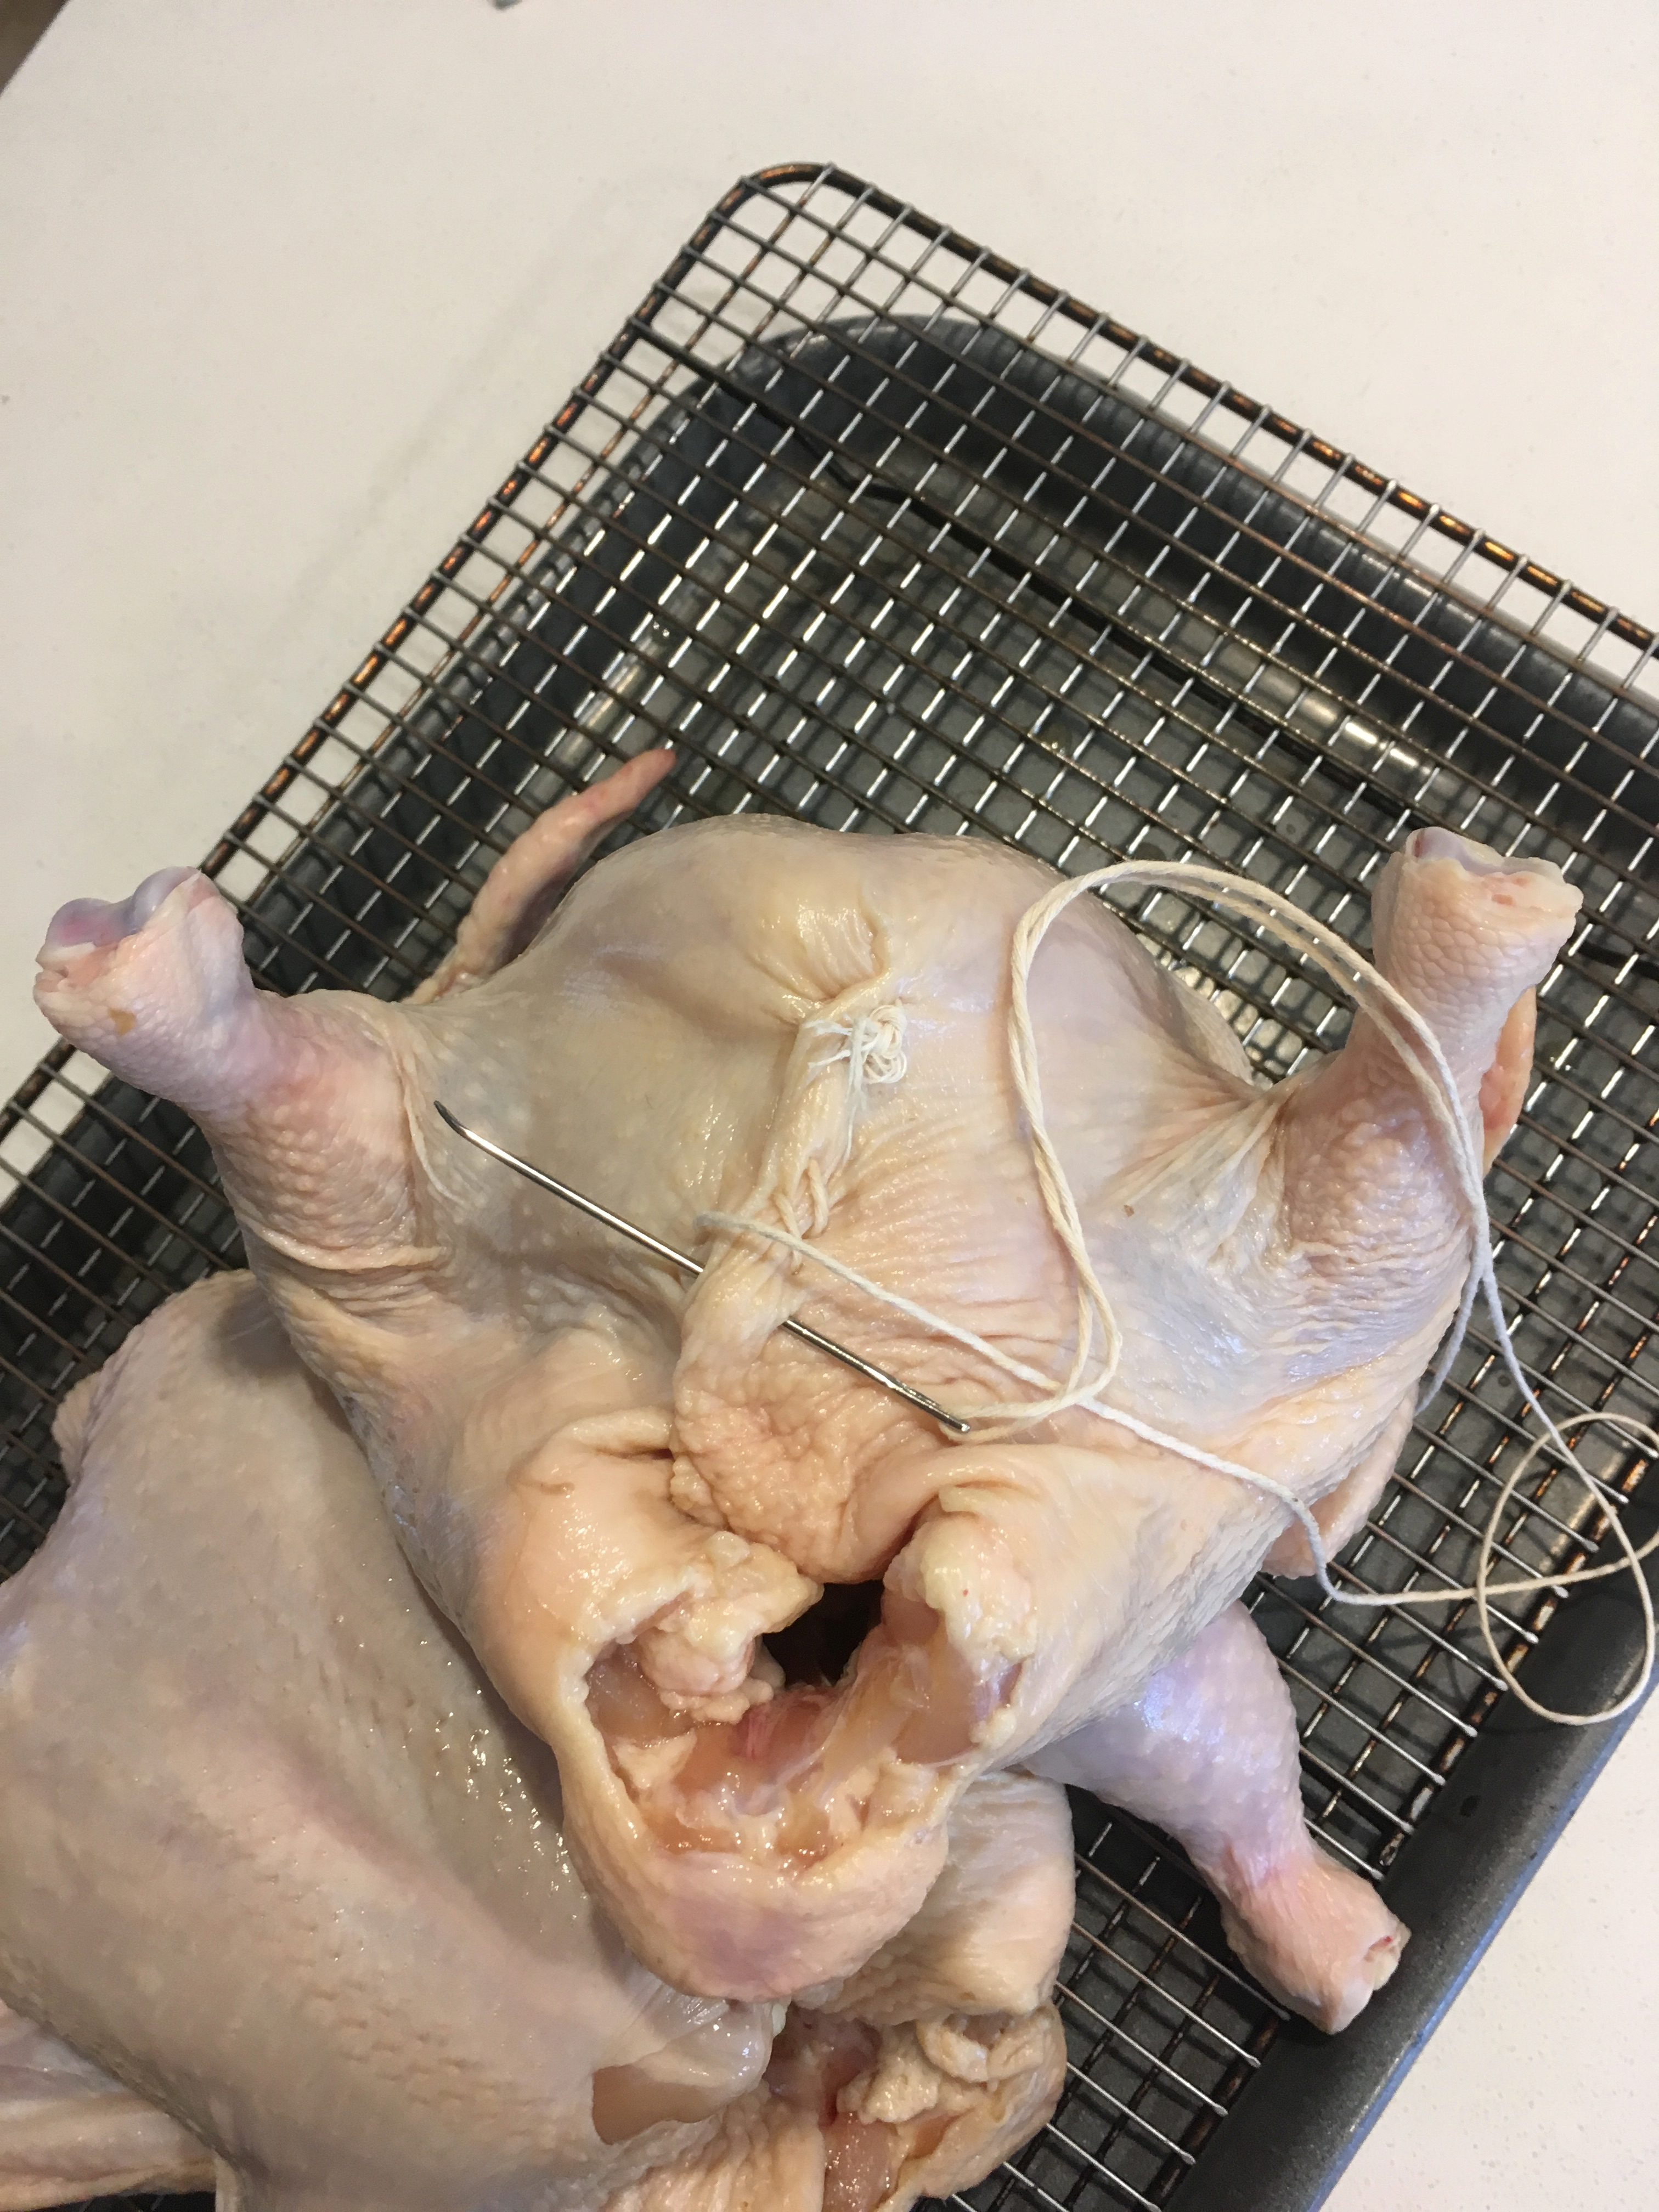
\includegraphics[width=0.25\textwidth]{\imageDir/\fileName/IMG_3216.jpg} \\
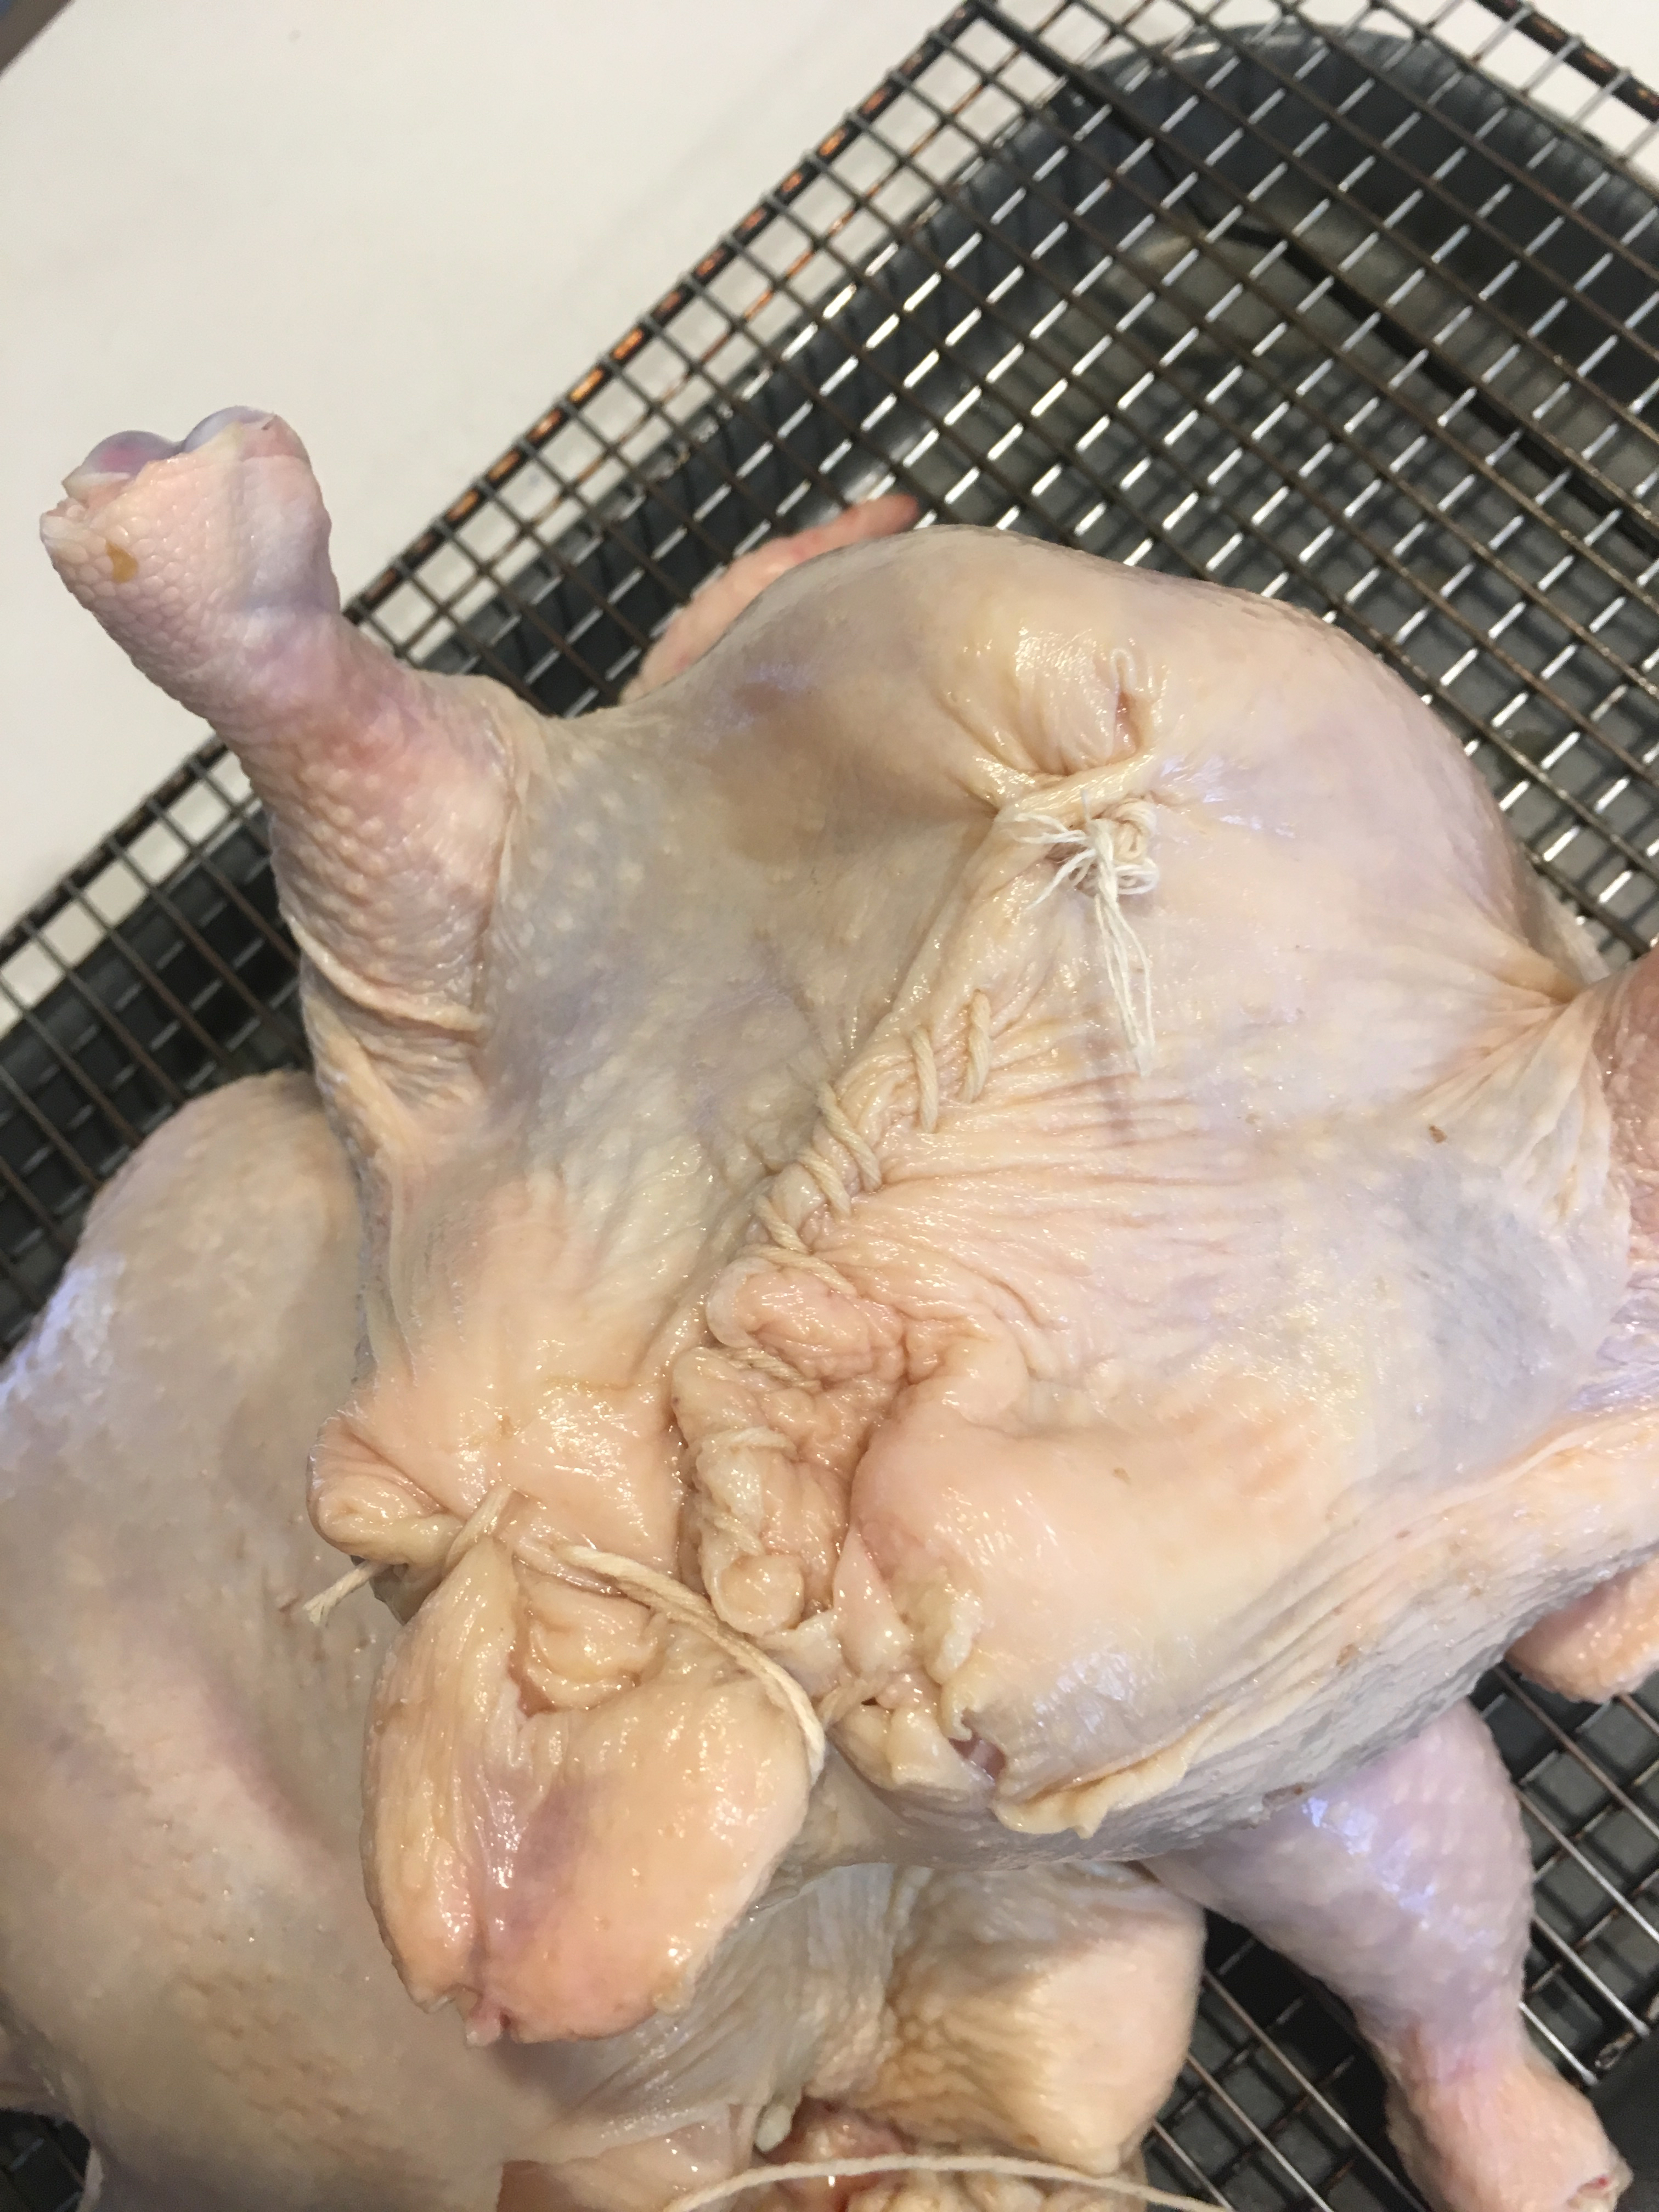
\includegraphics[width=0.25\textwidth]{\imageDir/\fileName/IMG_3217.jpg} &
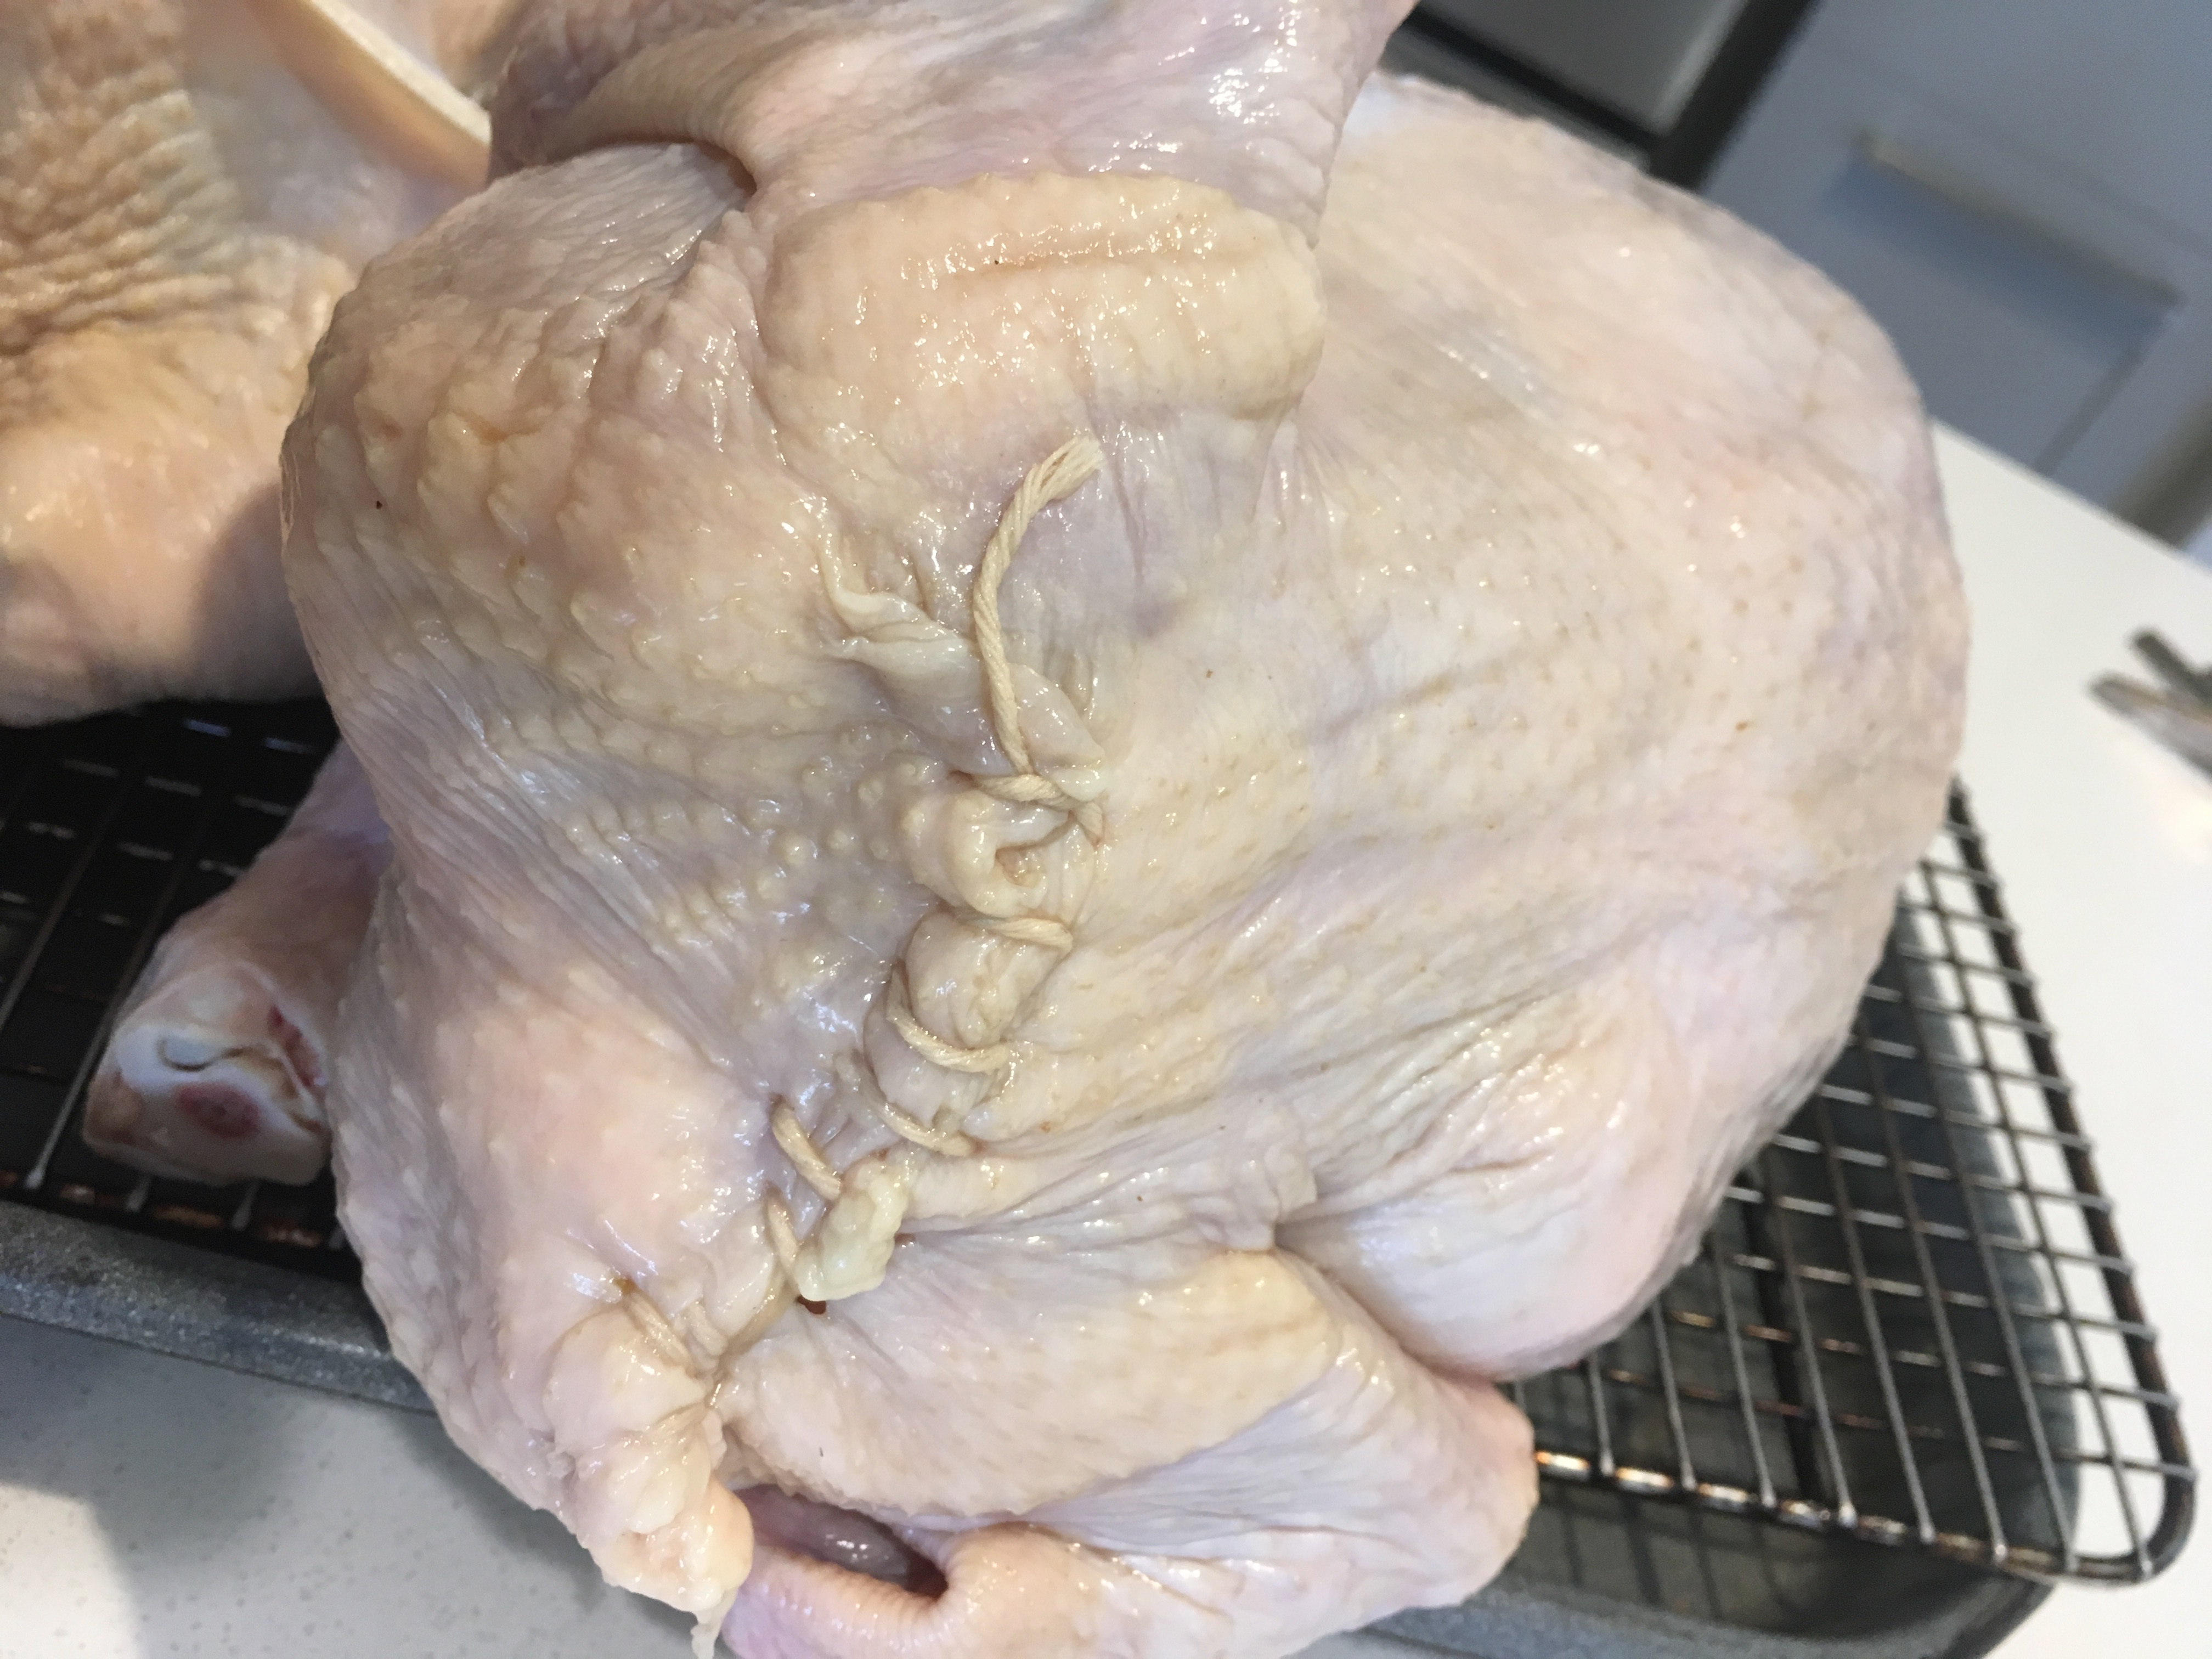
\includegraphics[width=0.25\textwidth]{\imageDir/\fileName/IMG_3218.jpg} &
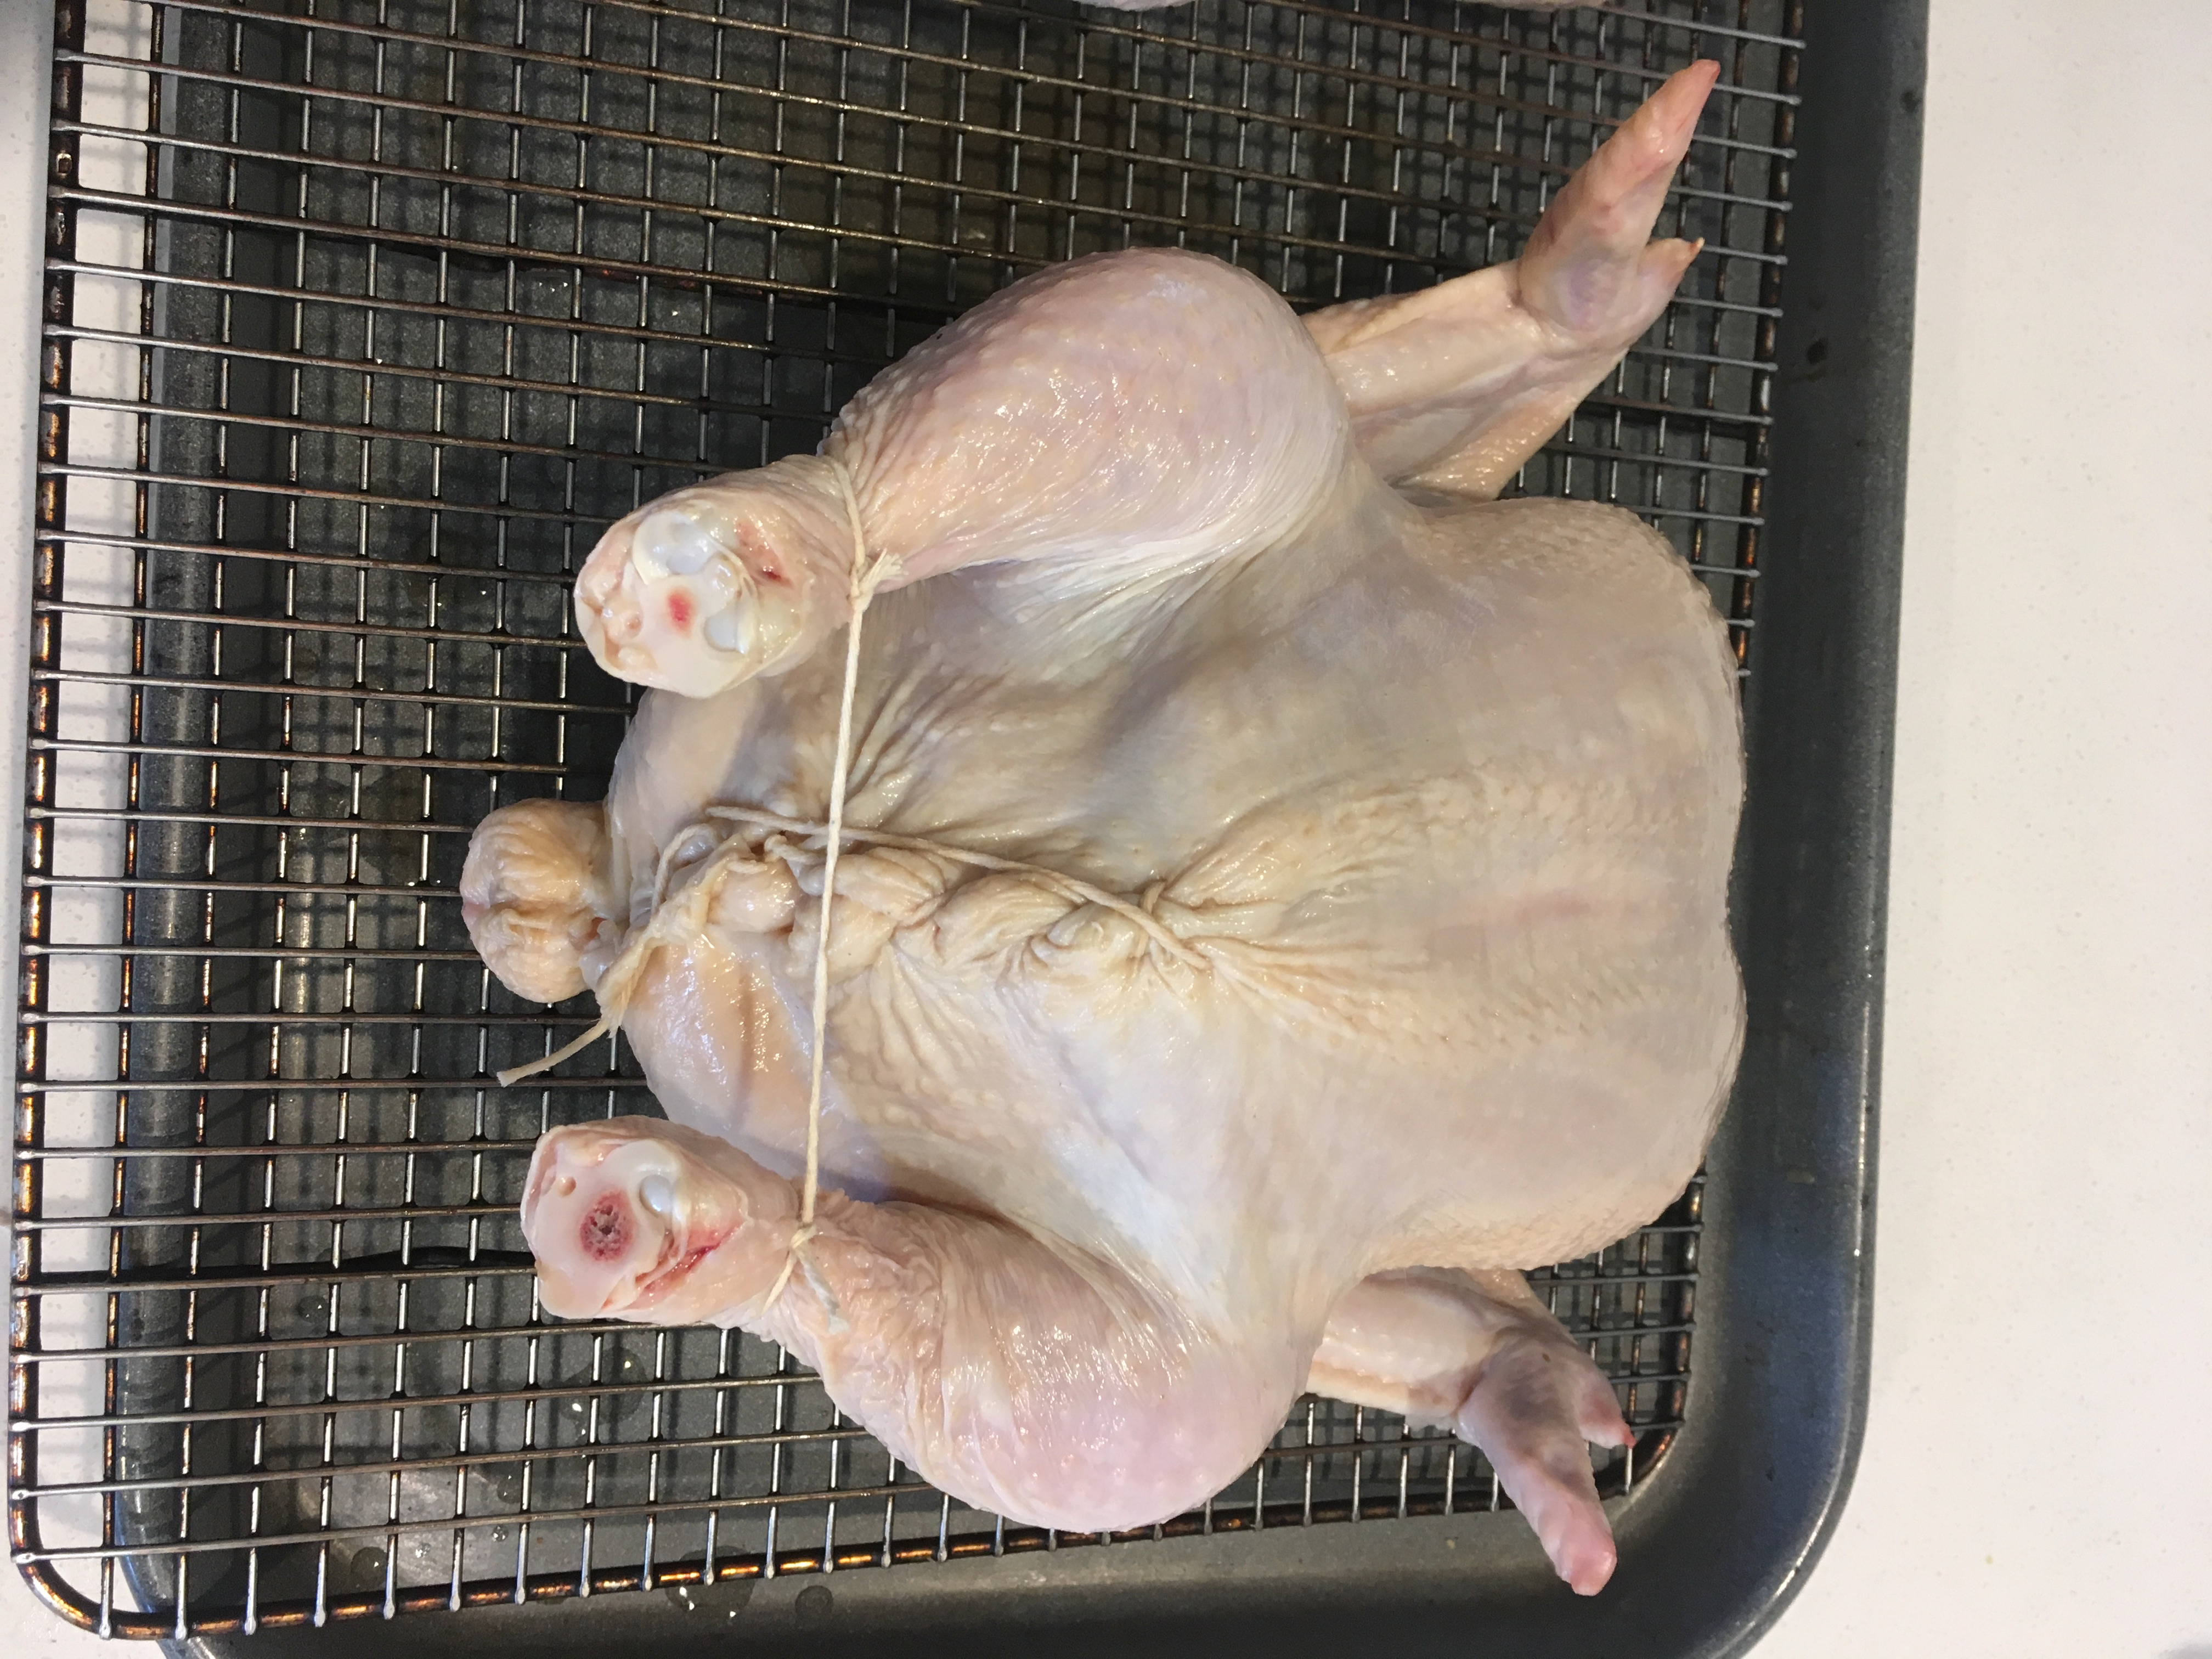
\includegraphics[width=0.25\textwidth]{\imageDir/\fileName/IMG_3219.jpg} \\
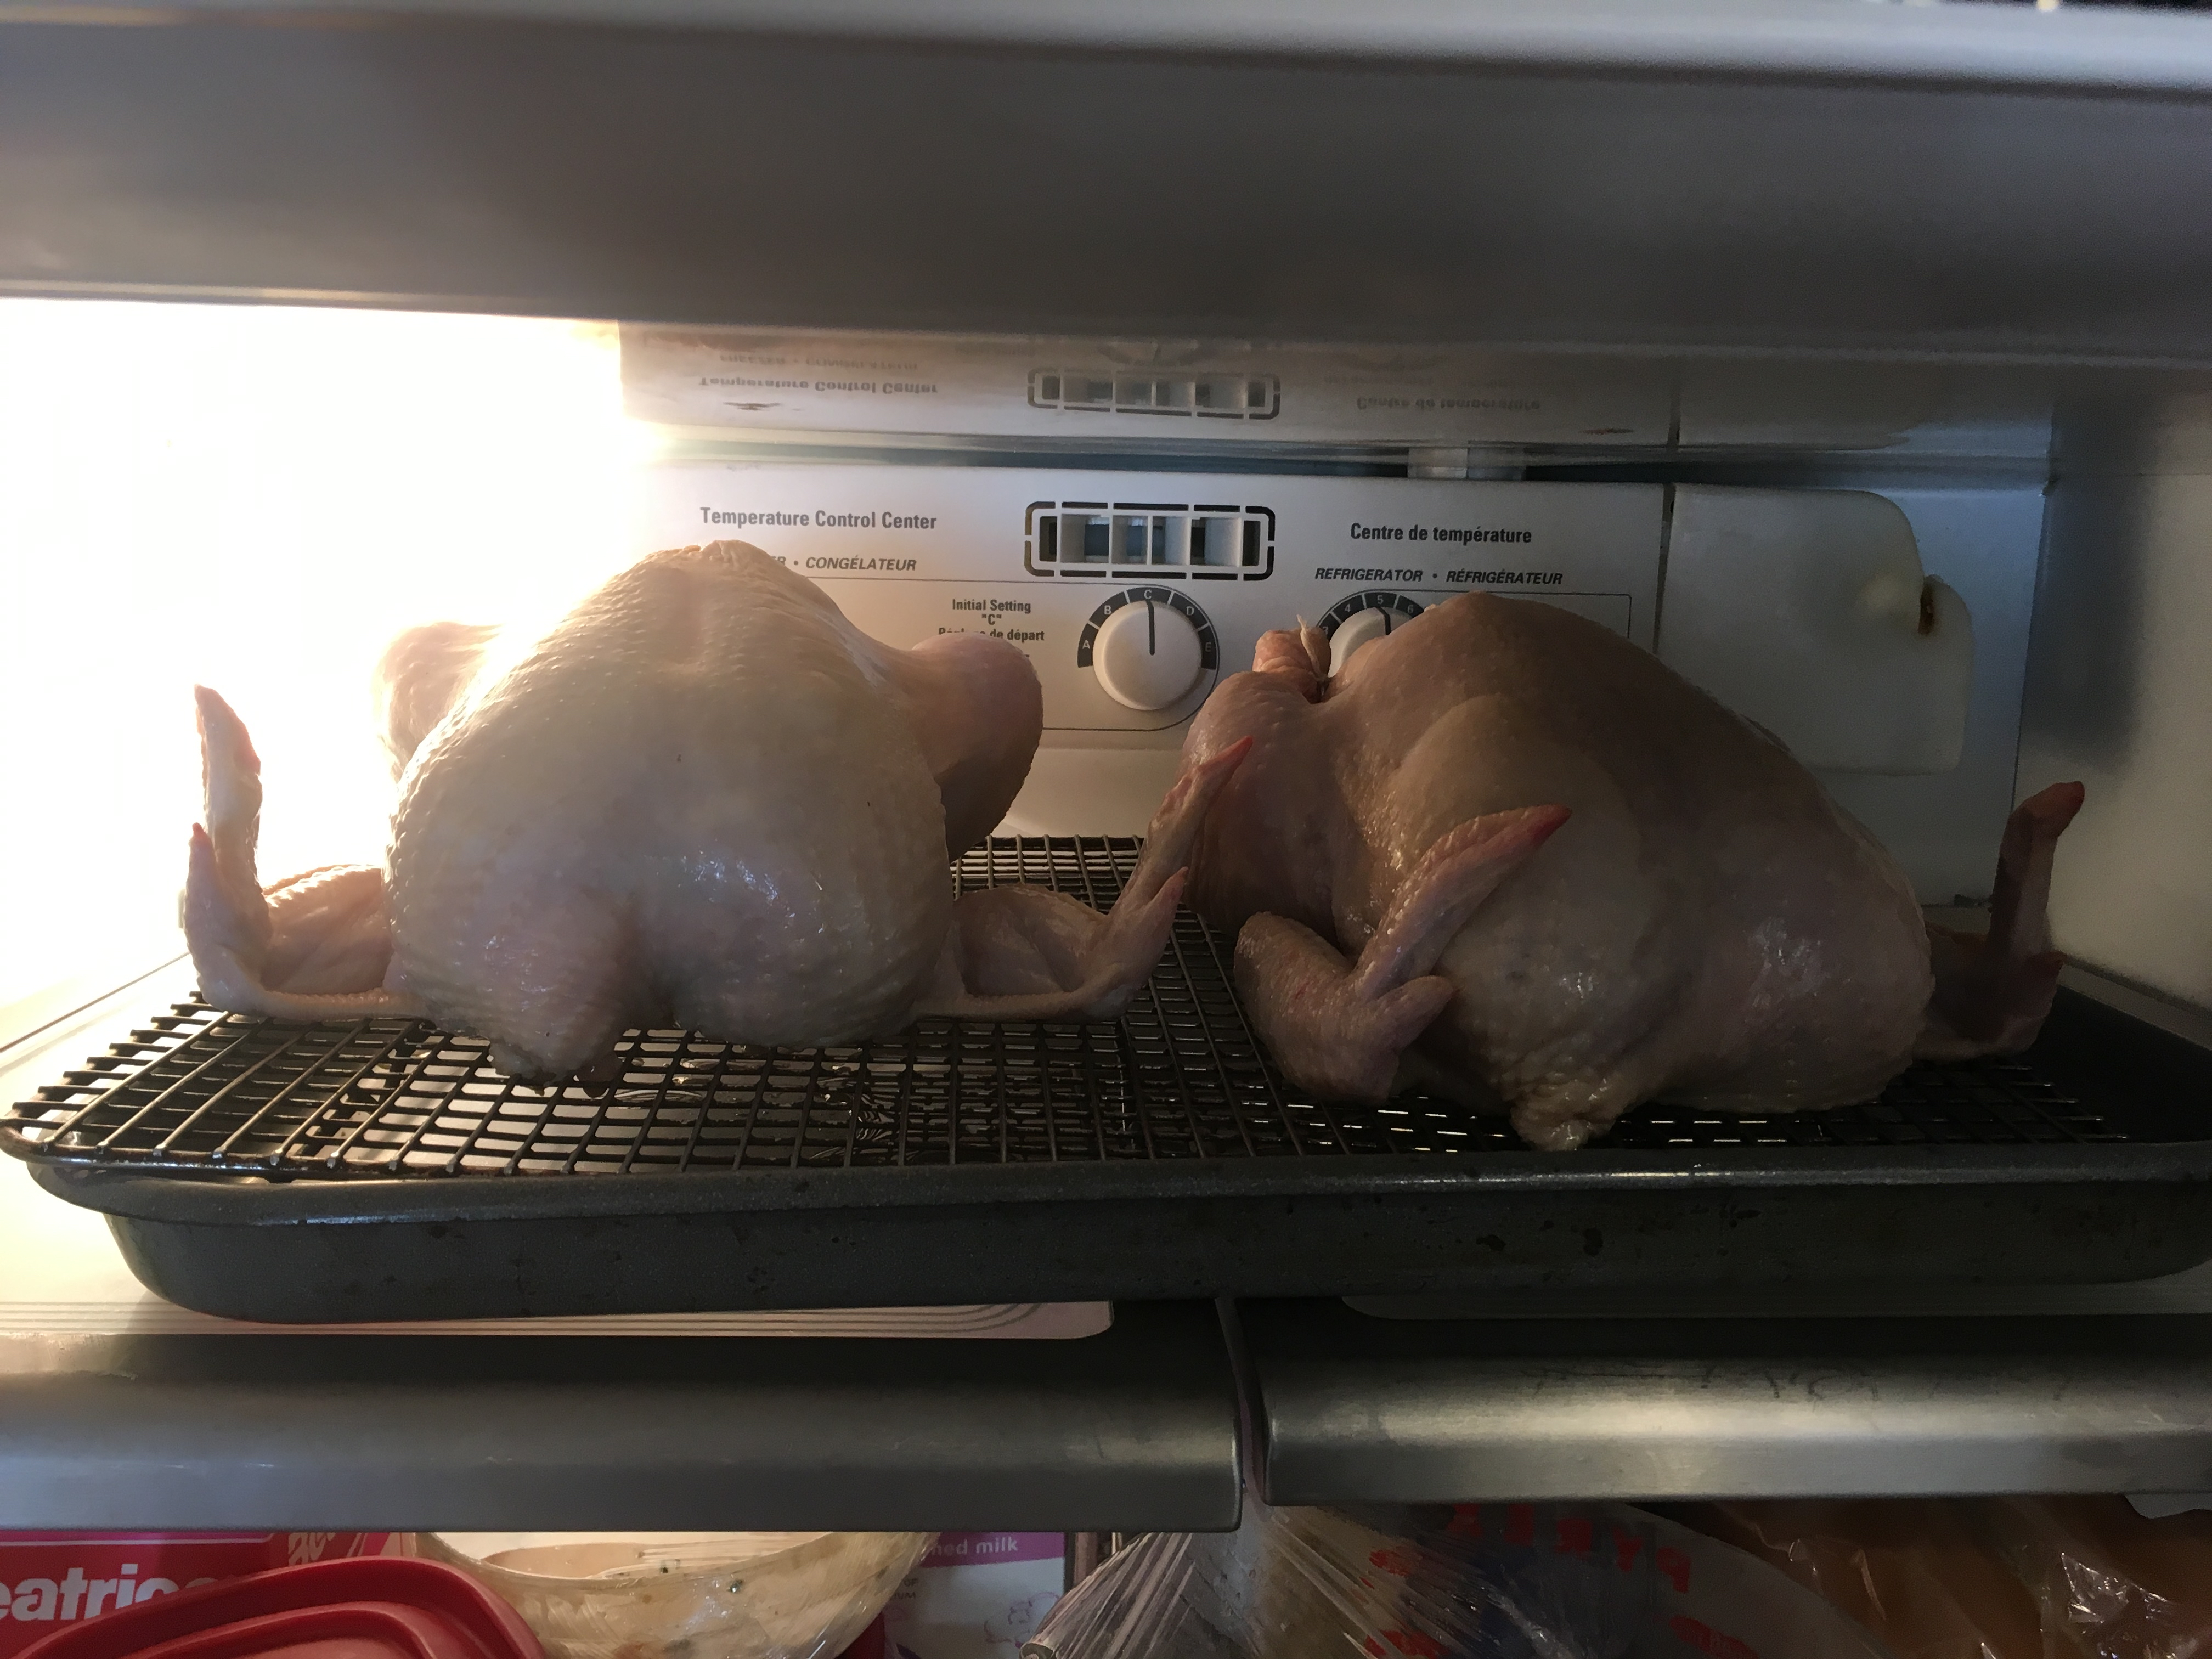
\includegraphics[width=0.25\textwidth]{\imageDir/\fileName/IMG_3220.jpg} &
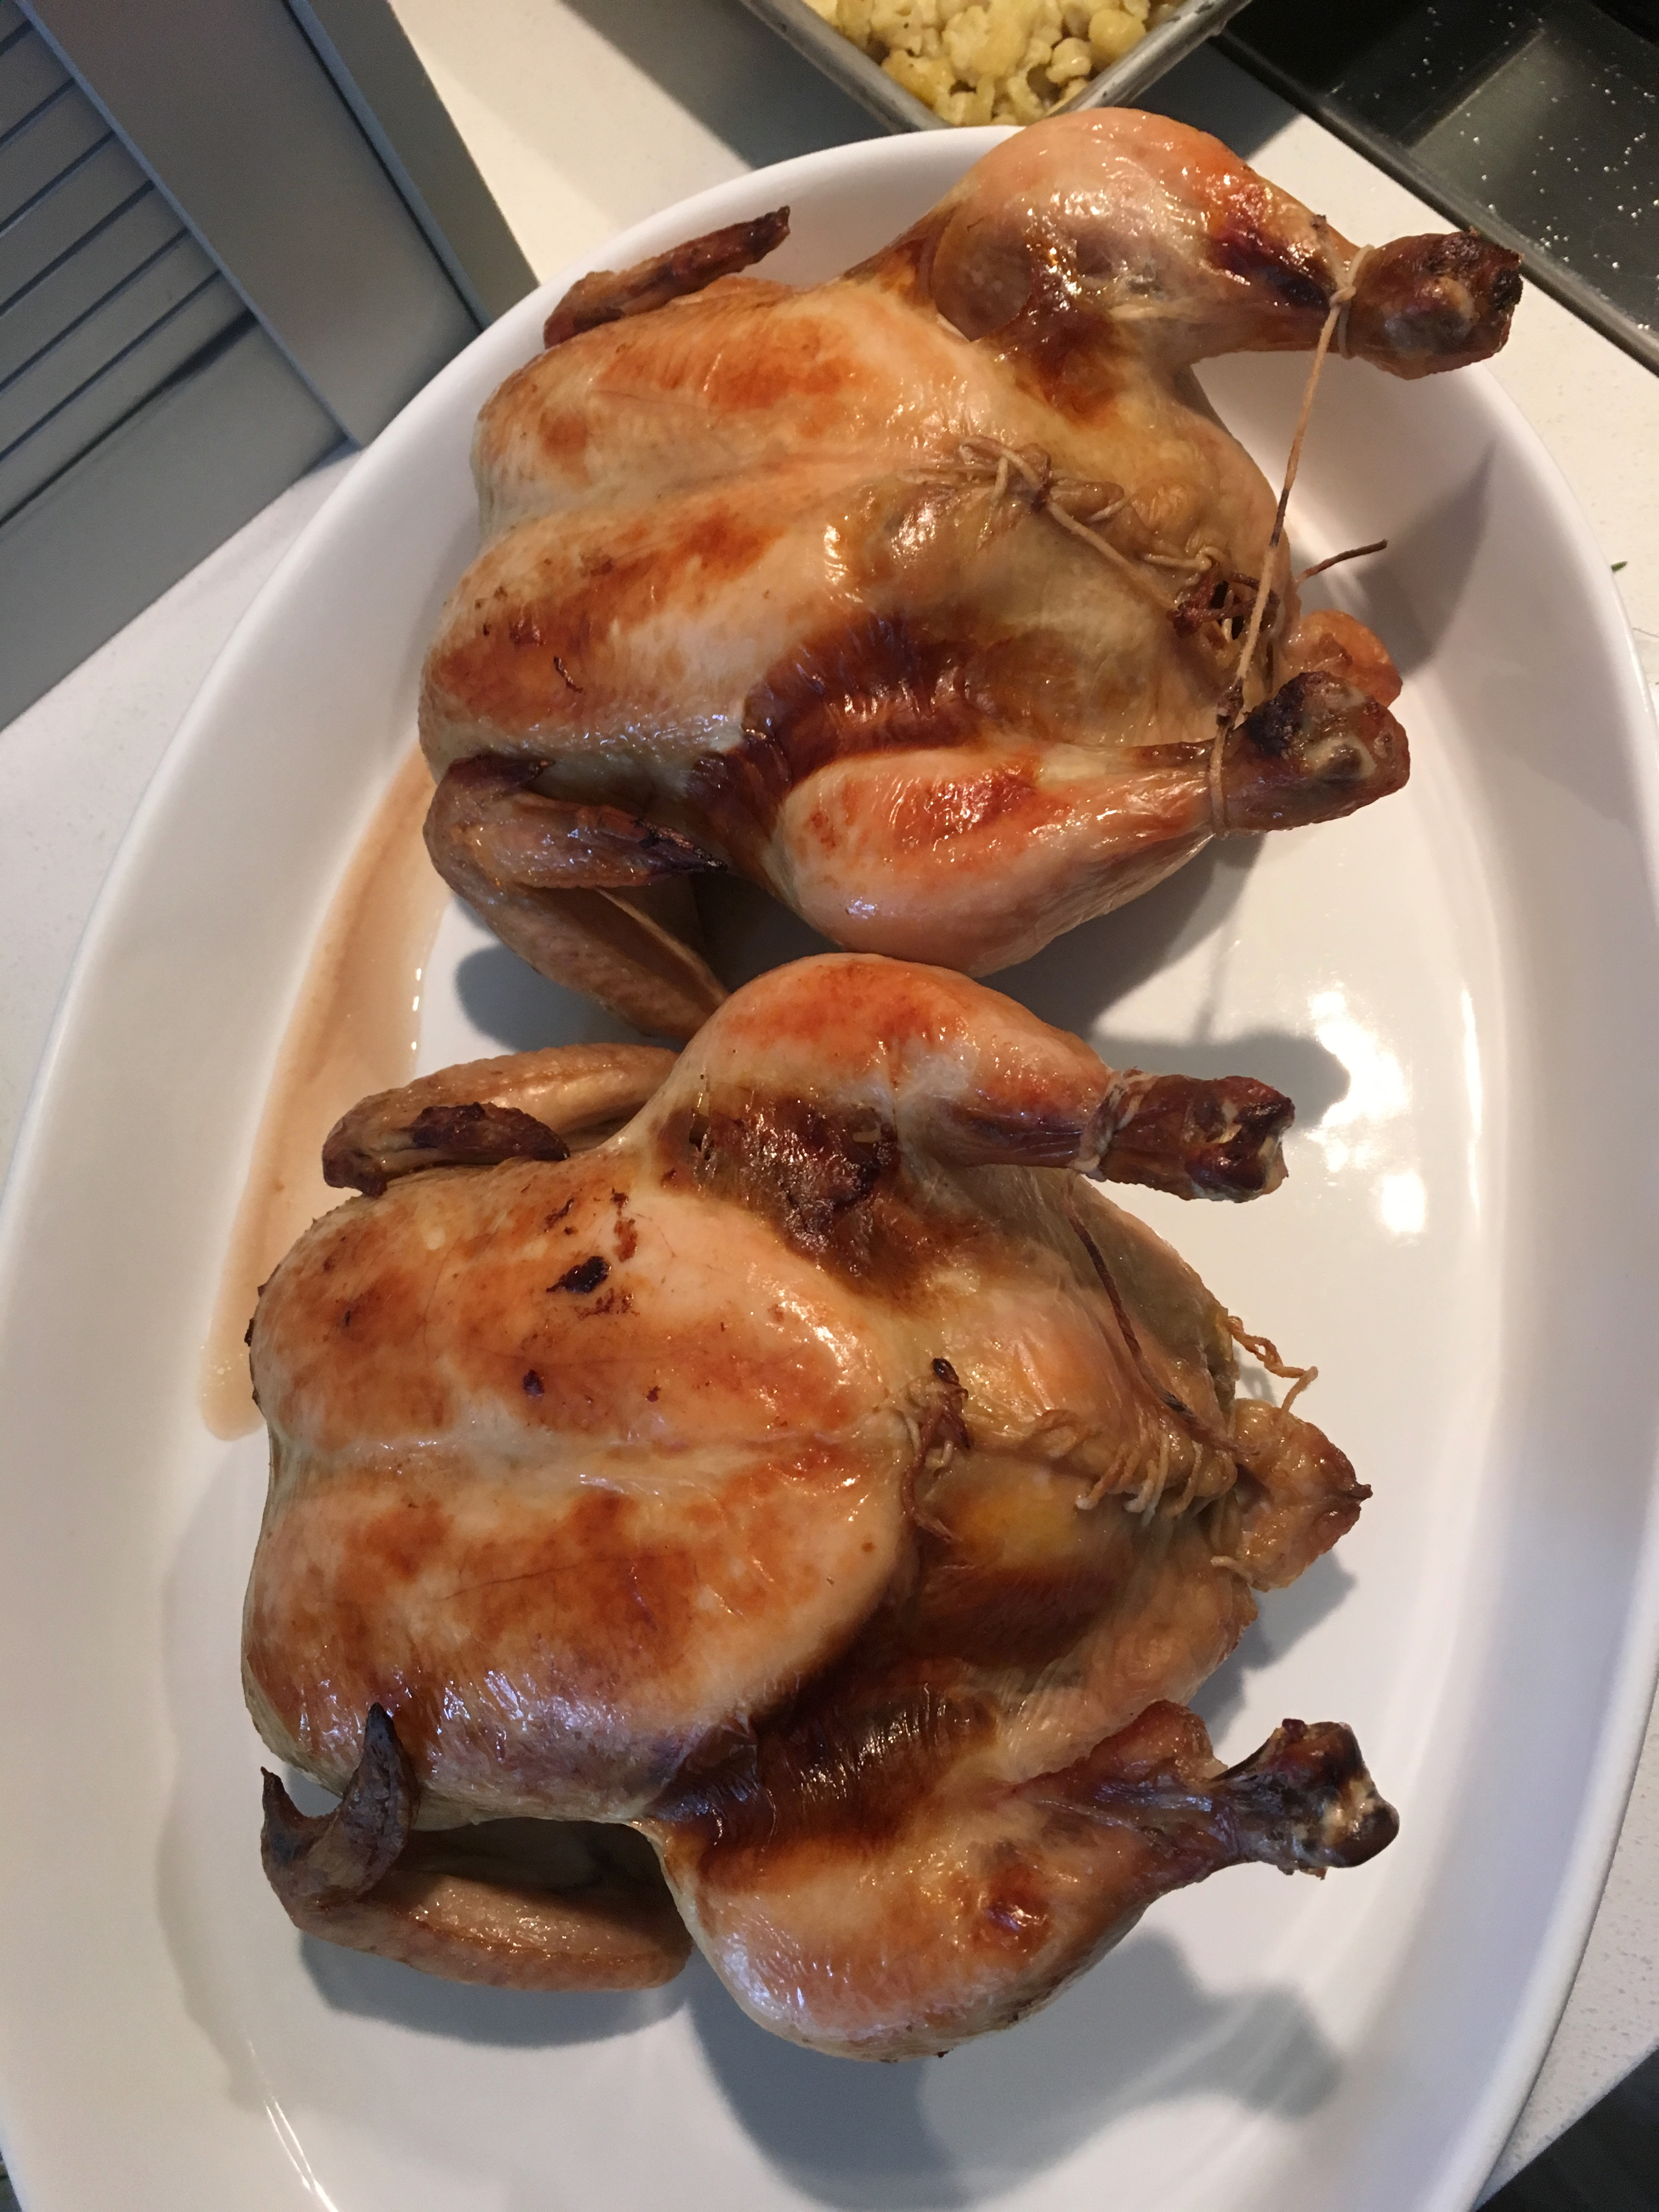
\includegraphics[width=0.25\textwidth]{\imageDir/\fileName/IMG_3228.jpg} \\
\end{tabular}
\end{table}

\end{document}
